\documentclass[11pt,twoside]{memoireuqam1.3}

\usepackage{todonotes}
\usepackage{amsmath}
\usepackage{amsthm}
\usepackage{amsfonts}
\usepackage{amssymb}
\usepackage{graphicx}
\usepackage[utf8x]{inputenc}
\usepackage[T1]{fontenc}
\usepackage[ocr-b]{ocr}
\usepackage[french]{babel}
\usepackage{subcaption}
\usepackage{captcont}
\usepackage{float}
\usepackage{tikz}
\usetikzlibrary{trees,backgrounds, calc, positioning, shapes, matrix}
\usepackage{xspace} % Pour ajouter un espace a une commande voir \noir et \blanc
\usepackage{csquotes}
\usepackage{array}
\usepackage{pgfplots}
\usepackage{pgfplotstable}
\usepackage{comment}
\usepackage{relsize}
\usepackage{mathtools}
\usepackage{algorithm}
\usepackage[noend]{algpseudocode}
\usepackage{pdfpages}
\usepackage{adjustbox}
\usepackage{enumitem}
\usepackage{listings}

% Blocs théorèmes
\newtheorem{definition}{Définition}
\newtheorem*{definition*}{Définition}
\newtheorem{proposition}{Proposition}
\newtheorem*{proposition*}{Proposition}
\newtheorem{theorem}{Théorème}
\newtheorem{lemma}{Lemme}
\newtheorem*{exercice*}{Exercice}
\newtheorem*{exemple*}{Exemple}
\newenvironment{preuve}{{\bf Preuve.}}{\hfill$\qed$}
\newenvironment{demonstration}{{\bf Démonstration.}}{$\qed$}


% Todos
\newcommand{\todoalex}[1]{\todo[inline]{Alexandre : #1}}
\newcommand{\todojerome}[1]{\todo[inline, color=green]{Jérôme : #1}}

% Macros
% !TEX root = memoire.tex

\tikzset{tuile/.style={draw, blue!60!black, fill=blue!10, minimum size=1cm, inner sep=0, outer sep=0}}
\newcommand{\tuile}[2][]{\node[tuile] at (#2) {#1}}

%\tikzset{point/.style={draw, circle, fill, inner sep=0.6mm}}
%\newcommand{\point}[1]{\node[point] at (#1) {}}
\newcommand{\point}[1]{\fill (#1) circle (3pt)}

\tikzset{pas/.style={auto, >=latex}}
\newcommand{\pas}[2]{\draw[pas] (#1) edge[->, bend left] (#2)}

% Typesetting gomino
\newcommand{\noir}{{\bf N}\xspace}
\newcommand{\blanc}{{\bf B}\xspace}

% Typesetting de Go

% Goban coté gauche
\newcommand{\goban}[2]{ 
	\clip (-0.7, -0.7) rectangle (#1.7-1,#2.7-1); 
	\fill[color=brown] (-0.7,-0.7) rectangle (#1,#2); 
	\draw (0,-1) grid (#1,#2+1); 
}

% Gobal central
\newcommand{\gobanc}[2]{ 
	\clip (-0.7, -0.7) rectangle (#1.7-1,#2.7-1); 
	\fill[color=brown] (-0.7,-0.7) rectangle (#1,#2); 
	\draw (-1,-1) grid (#1+1,#2+1); 
}

\newcommand{\kifu}[3][scale=.4]{
\begin{tikzpicture}[#1, every node/.style={#1, minimum size=1cm}, node distance=1cm]
\goban{#2}{#2}
#3
\end{tikzpicture}
}

\newcommand{\kifuc}[3][scale=1]{
\begin{tikzpicture}[#1, every node/.style={#1, minimum size=1cm}, node distance=1cm]
\gobanc{#2}{#2}
#3
\end{tikzpicture}
}


\newcommand{\woodgoban}[2]{
% parameters for the "wooden rectangle", chosen to be measures of a Go board
	\pgfmathsetmacro{\boardwidth}{#1}
	\pgfmathsetmacro{\boardheight}{#2}
	\pgfmathsetmacro{\relativefibrethickness}{0.10}
	\pgfmathsetmacro{\relativefibrevariation}{0.07}
	\pgfmathsetmacro{\numberoffibres}{(\boardwidth*5)} %20
	\pgfmathsetmacro{\fibresteps}{(\boardheight*5)} %10
	\newcommand{\backgroundcolor}{brown!95!yellow}
	\newcommand{\fibrecolor}{brown!95!black}

    %auto generated wood board  
	\clip (-0.7, -0.7) rectangle (\boardwidth + 0.7-1,\boardheight + 0.7-1); 

    \filldraw[\backgroundcolor] (-0.7, -0.7) rectangle (\boardwidth +0.7-1,\boardheight +0.7-1);

    \pgfmathsetmacro{\segmentwidth}{(\boardwidth + 0.7)/(\numberoffibres+1)}
    \pgfmathsetmacro{\segmentvariation}{\relativefibrethickness/2*\segmentwidth}

    \pgfmathsetmacro{\secondfibre}{2*\segmentwidth}
    \pgfmathsetmacro{\lastfibre}{\numberoffibres*\segmentwidth}

    \pgfmathsetmacro{\stepheight}{(\boardheight + 0.7)/\fibresteps}

	\begin{scope}[rotate=-2]
    \foreach \x in {0,...,\numberoffibres}
    {   \fill[\fibrecolor]
    			($(\x*\segmentwidth-\segmentvariation-0.7,0-0.7) + (rand*\relativefibrevariation*\relativefibrethickness,0)$) 
        
        		\foreach \y in {0,...,\fibresteps}
        		{
        			-- ($(\x*\segmentwidth-\segmentvariation-0.7,\y*\stepheight-0.7) + (rand*\relativefibrevariation*\relativefibrethickness,0)$)
        		}

	        -- ($(\x*\segmentwidth+\segmentvariation-0.7,\boardheight-0.7)+ (rand*\relativefibrevariation*\relativefibrethickness,0)$) 
    		    
    		    \foreach \y in {\fibresteps,...,0}
        		{   
        			-- ($(\x*\segmentwidth+\segmentvariation-0.7,\y*\stepheight-0.7) + (rand*\relativefibrevariation*\relativefibrethickness,0)$)
        		}
        -- cycle;
    }
    \end{scope}
	\draw (0,-1) grid (#1,#2+1); 
}


% Pierres
\newsavebox{\blackstonebox}
\savebox{\blackstonebox}{
	\begin{tikzpicture}
	\begin{scope}     	
		\fill[black] (0,0) circle (0.45);     	
		\clip (0,0) circle (0.45);     	
		\shade[outer color=black, inner color=black!30] (-0.15,0.5) circle (0.7); 	
	\end{scope}         
	\end{tikzpicture} 
}

\newsavebox{\whitestonebox}
\savebox{\whitestonebox}{
	\begin{tikzpicture}
	\begin{scope}     	
		\fill[white!80!black] (0,0) circle (0.45);   
		\clip (0,0) circle (0.45);     	
		\shade[outer color=white!80!black, inner color=white] (-0.15,0.5) circle (0.7); 	
	\end{scope}         
	\end{tikzpicture} 
}

\newsavebox{\redstonebox}
\savebox{\redstonebox}{
	\begin{tikzpicture}
	\begin{scope}        
		\fill[red] (0,0) circle (0.45);        
		\clip (0,0) circle (0.45);        
		\shade[outer color=red, inner color=red!30] (-0.15,0.5) circle (0.7);        
	\end{scope}
	\end{tikzpicture}
}

\newsavebox{\customwalkbox}
\savebox{\customwalkbox}{
	\begin{tikzpicture}
	\fill (0,0) rectangle (1,1);
	\end{tikzpicture}
}

\newcommand{\blackstone}{ \usebox{\blackstonebox} }
\newcommand{\whitestone}{ \usebox{\whitestonebox} }
\newcommand{\redstone}{ \usebox{\redstonebox} }
\newcommand{\customwalknode}{\usebox{\customwalkbox}}

\newcommand{\bm}[2][]{ \node at #2 {\blackstone}; \node at #2 {\color{white} #1}; }
\newcommand{\wm}[2][]{ \node at #2 {\whitestone}; \node at #2 {\color{black} #1};}


\usepackage{etextools}

% Using etextools, create a parser without delimiters that will 
% tokenize and process each letter one by one
\DeclareListParser*{\wordpath}{}

% Our substitution to convert the word to a TikZ path
\newcommand\BlackWalkParser[1]{
\ifcase \gettokslistindex{#1}{01234567} 
{--++(1,0) node{\blackstone} }
\or {--++(1,1) node{\blackstone} }
\or {--++(0,1) node{\blackstone} }
\or {--++(-1,1) node{\blackstone} }
\or {--++(-1,0) node{\blackstone} }
\or {--++(-1,-1) node{\blackstone} }
\or {--++(0,-1) node{\blackstone} }
\or {--++(1,-1) node{\blackstone} }
\fi}

\newcommand\WhiteWalkParser[1]{
\ifcase \gettokslistindex{#1}{01234567} 
{--++(1,0) node{\whitestone} }
\or {--++(1,1) node{\whitestone} }
\or {--++(0,1) node{\whitestone} }
\or {--++(-1,1) node{\whitestone} }
\or {--++(-1,0) node{\whitestone} }
\or {--++(-1,-1) node{\whitestone} }
\or {--++(0,-1) node{\whitestone} }
\or {--++(1,-1) node{\whitestone} }
\fi}

\newcommand\CustomWalkParser[1]{
\ifcase \gettokslistindex{#1}{01234567} 
{--++(1,0) node{\customwalknode} }
\or {--++(1,1) node{\customwalknode} }
\or {--++(0,1) node{\customwalknode} }
\or {--++(-1,1) node{\customwalknode} }
\or {--++(-1,0) node{\customwalknode} }
\or {--++(-1,-1) node{\customwalknode} }
\or {--++(0,-1) node{\customwalknode} }
\or {--++(1,-1) node{\customwalknode} }
\fi}

\newcommand\SimplePathParser[1]{
\ifcase \gettokslistindex{#1}{01234567} 
{--++(1,0)}
\or {--++(1,1)}
\or {--++(0,1)}
\or {--++(-1,1)}
\or {--++(-1,0)}
\or {--++(-1,-1)}
\or {--++(0,-1)}
\or {--++(1,-1)}
\fi}


% a command to invoke the parser and do the substitution
\newcommand\blackwalk[1]{\wordpath{\BlackWalkParser}{#1}}
\newcommand\whitewalk[1]{\wordpath{\WhiteWalkParser}{#1}}
\newcommand\customwalk[1]{\wordpath{\CustomWalkParser}{#1}}
\newcommand\simplewalk[1]{\wordpath{\SimplePathParser}{#1}}

% one-step parsing/drawing.
\newcommand\whitestonepath[2]{
	\edef\tmp{\whitewalk{#2}};
	\path #1 node{\whitestone} \tmp;
}

\newcommand\blackstonepath[2]{
	\edef\tmp{\blackwalk{#2}};
	\path #1 node{\blackstone} \tmp;
}

\newcommand\custompath[2]{
	\edef\tmp{\customwalk{#2}};
	\path #1 node{\customwalknode} \tmp;
}


\newcommand{\squarepath}[3][blue]{
	\savebox{\customwalkbox}{\draw[#1!60!black, fill=#1!10] (0,0) rectangle (1,1);}
	\custompath{#2}{#3};
}

\newcommand\simplepath[3][]{
	\edef\tmp{\simplewalk{#3}};
	\draw[#1] #2 \tmp;
}

\newcommand{\expandboundingbox}{\node[inner sep=0] at ($(current bounding box.north east) + (1,1)$) {};}
\newcommand{\polyomino}[2][blue]{
\begin{tikzpicture}[fill=red]
\squarepath[#1]{(0,0)}{#2}
\expandboundingbox
\end{tikzpicture}
}

%
% Example
%
%\begin{tikzpicture}
%\squarewalk{(0,1)}{000222};
%\squarewalk[red]{(0,0)}{00066};
%\end{tikzpicture}

% Paul Gaborit
% http://tex.findincity.net/view/635399273629833626147690/tikz-radial-shading-of-a-ring
\tikzset{
  ring shading/.code args={from #1 at #2 to #3 at #4}{
    \pgfmathsetmacro{\inner}{25*#2/#4}
    \pgfmathsetmacro{\innerlow}{\inner-1}
    \pgfdeclareradialshading{ring}{\pgfpoint{0cm}{0cm}}%
    {
      color(0bp)=(white);
      color(\innerlow bp)=(white);
      color(\inner bp)=(#1);
      color(25bp)=(#3);
      color(50bp)=(black)
    }
    \pgfkeysalso{/tikz/shading=ring}
  },
}

\pgfdeclareradialshading{stoneshading}{\pgfpointorigin}
{
  color(0mm)=(pgftransparent!100);
  color(0.45cm)=(pgftransparent!0);
  color(0.4501cm)=(pgftransparent!30);
  color(.6cm)=(pgftransparent!100)
}
\pgfdeclarefading{stonemarking}{\pgfuseshading{stoneshading}}
\pgfdeclarefading{fading3}{\pgfuseshading{stoneshading}}

\newcommand{\markstone}[3][green]{
\begin{scope}
\pgfsetfading{stonemarking}{\pgftransformshift{\pgfpoint{#2cm}{#3cm}}};
\fill [#1, even odd rule] (#2, #3) circle (.6) circle (.45);
\end{scope}
}
\newcommand{\N}{\mathbb{N}}
\newcommand{\Z}{\mathbb{Z}}
\newcommand{\R}{\mathbb{R}}
\newcommand{\A}{\mathcal{A}}
\newcommand{\F}{\mathcal{F}}
\renewcommand{\O}{\mathcal{O}}
% notation "such that" { (x,y) \st x^2+y^2=0 }
\newcommand{\st}{\mathrel{}\middle|\mathrel{}}

\newcommand{\verifier}[1]{{\color{red} #1}}
\newcommand{\Go}{\mbox{\em go}\xspace}

\newcommand{\B}{\mathbf{B}}
\newcommand{\W}{\mathbf{W}}

\newcommand{\thickhline}{\noalign{\hrule height 0.8pt}}
\newcommand{\thickvline}{\vrule width .8pt}

\newcommand{\conv}[1]{\text{Conv}(#1)}

% Nombres encerclés
% http://tex.stackexchange.com/questions/7032/good-way-to-make-textcircled-numbers
\newcommand*\circled[1]{\tikz[baseline=(char.base)]{
            \node[shape=circle,draw,inner sep=1.5pt] (char) {#1};}}

\DeclarePairedDelimiter\ceil{\lceil}{\rceil}
\DeclarePairedDelimiter\floor{\lfloor}{\rfloor}


% Traductions d'algorithmes
\floatname{algorithm}{Algorithme}
\renewcommand{\algorithmicrequire}{\textbf{Préconditions:}}
\renewcommand{\algorithmicensure}{\textbf{Postconditions:}}
\renewcommand{\algorithmicend}{\textbf{fin}}
\renewcommand{\algorithmicif}{\textbf{si}}
\renewcommand{\algorithmicthen}{\textbf{alors}}
\renewcommand{\algorithmicelse}{\textbf{sinon}}
\renewcommand{\algorithmicfor}{\textbf{pour}}
\renewcommand{\algorithmicforall}{\textbf{pour tout }}
\renewcommand{\algorithmicdo}{\textbf{faire}}
\renewcommand{\algorithmicwhile}{\textbf{tant que}}
\renewcommand{\algorithmicreturn}{\textbf{retourner}}


%\usepackage{hyperref}
\usepackage{url}
\newcommand{\href}[1]{\url{#1}}

\begin{document}

%%%%%%%%%%%%%%%%%%%%
% Pour la page titre
%%%%%%%%%%%%%%%%%%%%
\title{G\'en\'eration exhaustive de polyominos}
\author{J\'er\^ome Tremblay} % on doit utiliser les codes d'accents dans "author".
\degreemonth{Mai}
\degreeyear{2016}
\uqammemoire

\thispagestyle{empty}        % La page titre n'est pas numérotée
\maketitle

%%%%%%%%%%%%%%%%%%%%
% Page préliminaires
%%%%%%%%%%%%%%%%%%%%

\renewcommand \listfigurename{LISTE DES FIGURES}
\renewcommand \appendixname{APPENDICE}
\renewcommand \figurename{Figure}
\renewcommand \tablename{Tableau}

\pagenumbering{roman} % numérotation des pages en chiffres romains
\addtocounter{page}{1} % Pour que les remerciements commencent à la page ii

% !TEX root = memoire.tex
\section*{Remerciements}
Merci à mon directeur, Srečko, de m'avoir inlassablement poussé vers la réussite.
Merci à mes co-auteurs, Alain, Hugo, Jérôme, Jonathan et Romaine, d'avoir partagé mon aventure dans le merveilleux monde de la recherche fondamentale.
Merci à mon ange gardien, Johanne, de m'avoir écouté, réglé mes problèmes et de façon générale pensé à tout!
Merci à mes collègues, Alexandre, Alexandra, Anne, Christian, Christophe, Christophe, Franco, François, Gilbert, Gisèle, Manon, Steven, Steven, Sylvie et Vestislav, j'ai apprécié chaque jour de travail grâce à vous tous.
Merci à ma conscience, Marie-Claude, de m'avoir permis de survivre à la bureaucratie.
Merci à mes amis, Catherine, Didier, Hugues, Judith, Jean-Philippe, Malorie, Marco, Marie, Maxime, Nicolas, Nicolas, Sébastien et bien d'autres, d'avoir fait passer toutes ces années si rapidement.
Merci à ma douce, Catherine, de m'avoir soutenu et encouragé tout ce temps.
Merci à Pierre, de m'avoir ouvert les portes du LaCIM.

\tableofcontents % Pour générer la table des matières
\listoffigures % Pour générer la liste des figures
\listoftables % Pour générer la liste des tableaux
% !TEX root = memoire.tex
\begin{abstract}


La géométrie digitale est un domaine d'études développé récemment, à cause du  développement des outils numériques. 
Ce mémoire examine deux problèmes  importants dans le domaine de la géométrie digitale, à savoir le calcul de l’enveloppe extérieure d’un chemin discret et également la génération exhaustive de polyominos. Les deux reposent sur le codage des objets dans le plan discret, assimilé à la grille carrée $\Z\times\Z$, par des mots sur l'alphabet de Freeman $\F=\{\ocr{0},\ocr{1},\ocr{2},\ocr{3}\}$, correspondant aux déplacements élémentaires sur la grille carrée.

Pour le problème de l'enveloppe extérieure d'un chemin quelconque (se recoupant ou pas), on utilise une structure de données utilisant deux arbres quaternaires superposés, introduite par Brlek, Provençal et Koskas. Utilisant un parcours mimant l'algorithme de la main droite dans un labyrinthe on obtient un algorithme linéaire en temps et en espace pour effectuer le calcul de l'enveloppe extérieure.

Dans le cas de la génération de polyominos codés par un chemin décrivant leurs périmètres de site, on utilise une adaptation du jeu de go pour construire à partir de l'origine et dans le sens antihoraire le chemin qui les borne. L'algorithme est exhaustif, et génère un polyomino chaque fois que le joueur noir gagne.






\textit{Mots-clés:} polyominos, gominos, périmètre de site, chemins, enveloppe externe, génération exhaustive, algorithme, mots, arbre radix.

\end{abstract}


%%%%%%%%%%%%%%%%%%%%
% Document principal
%%%%%%%%%%%%%%%%%%%%

\parindent=0ex % Facultatif
% pour qu'il n'y ait pas  de renfoncement à chaque alinéa

% !TEX root = memoire.tex
\begin{introduction}

L'avènement des ordinateurs au cours des dernières décennies a apporté des changements technologiques qui ont bouleversé les communications, la transmission d'informations et le traitement des données numériques. 

En particulier, l'acquisition, la synthèse et le traitement des images constituent  aujourd'hui un champ d'activité fertile pour le développement de nombreuses applications qu'on voit dans la vie de tous les jours. Astronomie, médecine, météorologie, surveillance, vision, sécurité et même le transport sont autant de domaines qui bénéficient de ces avancées technologiques. 

Ces technologies sont basées sur des structures de données et algorithmes opérant sur une matrice de points (pixels) étudiés depuis longtemps et le corpus des connaissances acquises forme le coeur du domaine de la géométrie digitale. On s'accorde généralement pour situer la naissance de ce domaine en 1969 \cite{Rosenfeld69}, bien qu'on trouve des algorithmes pour tracer des segments de droite bien avant \cite{Bresenham65} ainsi que d'autres notions qui se sont avérées équivalentes \cite{Chrl1875}. 

Le plan de pixels s'identifie naturellement au plan discret constitué par le produit cartésien $\Z\times\Z$, et une figure discrète dans le plan n'est rien d'autre qu'un sous-ensemble de $\Z\times\Z$. Les figures connexes dans le plan discret sont commodément représentées par les chemins qui les bornent. Ainsi le bord est constitué par un chemin, ou plusieurs chemins si la figure possède des trous.

Le polyomino est une de ces figures discrètes. Popularisé par S. Golomb~\cite{dbintr39} comme jeu mathématique, le polyomino est un objet combinatoire rencontré dans plusieurs problèmes intéressants tels les pavages~\cite{BN, Golomb} ainsi que certains jeux~\cite{Ga} et problèmes d'énumération~\cite{Jen, JenGutt}. De plus, certaines classes de polyominos codent efficacement les partages d'entiers et sont utilisés en théorie des nombres et en physique mathématique pour représenter le groupe symétrique~\cite{fulton97}. Une représentation commode de tout polyomino est donc réalisée par les chemins qui le bornent.

%Ces objets sont particulièrement étudiés en géométrie digitale et en informatique théorique, les coordonnées entières se prêtant naturellement à l'adressage de composants électroniques distincts bien alignés sur une galette de silicium. 




Ce mémoire concerne deux problèmes importants dans le domaine de la géométrie digitale, à savoir le calcul de l'enveloppe extérieure d'un chemin discret et également la génération exhaustive de polyominos. 



%%%%%%%% Partie chemins %%%%%%%%%%%%
Les objets convexes tiennent un rôle important dans plusieurs branches des mathématiques, comme l'analyse fonctionnelle, l'optimisation, les probabilité et la physique mathématique (voir \cite{Gruber} pour un traitement détaillé de la géométrie convexe et ses applications.) En géométrie euclidienne, étant donné un ensemble fini de points, le problème de trouver le plus petit ensemble convexe les contenant tous a mené à l'introduction de la notion géométrique d'enveloppe convexe. Le calcul de l'enveloppe convexe s'est révélé être l'un des algorithme fondamental de la géométrie computationelle avec des applications allant de la recherche opérationelle \cite{Sherali199483} à l'automatisation du design \cite{kim}. Il est également largement utilisé en graphisme, en particulier dans le traitement d'images \cite{KimLee}. Il est bien connu que dans le cas euclidien, les algorithmes de calcul de l'enveloppe convexe d'un ensemble $S\subset \R^2$ s'exécutent en temps $\O(n\log n)$ où $n=|S|$ (voir \cite{Graham1972132, Chan96}). On peut même montrer que de tels algorithmes sont optimaux à une constante linéaire près \cite{Avis198281,Boas80}.

Néanmoins, en restreignant le problème au calcul de l'enveloppe convexe de polygones simples, une borne asymptotique linéaire est établie  \cite{McCallumAvis, Melkman87}. La version digitale de ce problème est un peu plus compliquée. On peut par exemple calculer l'enveloppe convexe d'un ensemble de pixels $S$ en commençant par calculer l'enveloppe convexe Euclidienne de $S$ et ensuite en digitalisant le résultat \cite{Chaudhuri98}. Ceci nous donne automatiquement un pire cas en $\O(n \log n)$. Dans le cas discret, la situation est surprenamment plus simple grâce à l'aide de la combinatoire des mots, qui a récemment mené au développement d'outils efficaces pour l'étude de la géométrie digitale \cite{thesexavier, blondin12}. Par exemple, des bornes asymptotiques linéaires ont été établues lorsqu'on considère un chemin discret codé par une suite de pas élémentaires. En effet, Brlek et al. ont développé un algorithme linéaire pour calculer l'enveloppe convexe discrète d'un chemin fermé auto-évitant sur la grille carré \cite{blpr09}. Il est basé sur un algorithme de Duval \cite{Duval83} linéaire en temps et en espace optimal pour factoriser un mot de Lyndon. La situation est plus compliquée dans le cas d'un chemin non-simple.

Au chapitre \ref{chapitre-chemins} nous présentons un algorithme linéaire en temps et en mémoire pour calculer l'enveloppe extérieure d'un chemin discret décrit par un mot sur le code de Freeman. L'utilisation d'une structure d'arbre radix augmenté \cite{BKP} permet une représentation linéaire des points visités ainsi que leur liens de voisinage dans le plan discret $\Z \times \Z$. Construire cette structure de données est une opération linéaire en temps et en espace et combinée à l'algorithme de la main droite, bien connu pour la résolution de labyrinthe, permet d'obtenir un algorithme linéaire en temps et en espace pour calculer l'enveloppe externe. Ce résultat fut exposé à la conférence Internationale <<18th IAPR International Conference, DGCI 2014, Siena, Italy, September 10-12, 2014.>>
\begin{quote}\setstretch{0.8} Brlek, S., Tremblay, H., Tremblay, J. et Weber, R. (2014). Efficient computation of the outer hull of a discrete path. Dans Discrete Geometry for Computer Imagery -
 Proceedings, volume 8668 de Lecture Notes in Computer Science. 
\end{quote}

%%%%%%%% Polyominos %%%%%%%%%%%%


%\ref{scamp3}.
 
%\begin{figure}
%\centering
%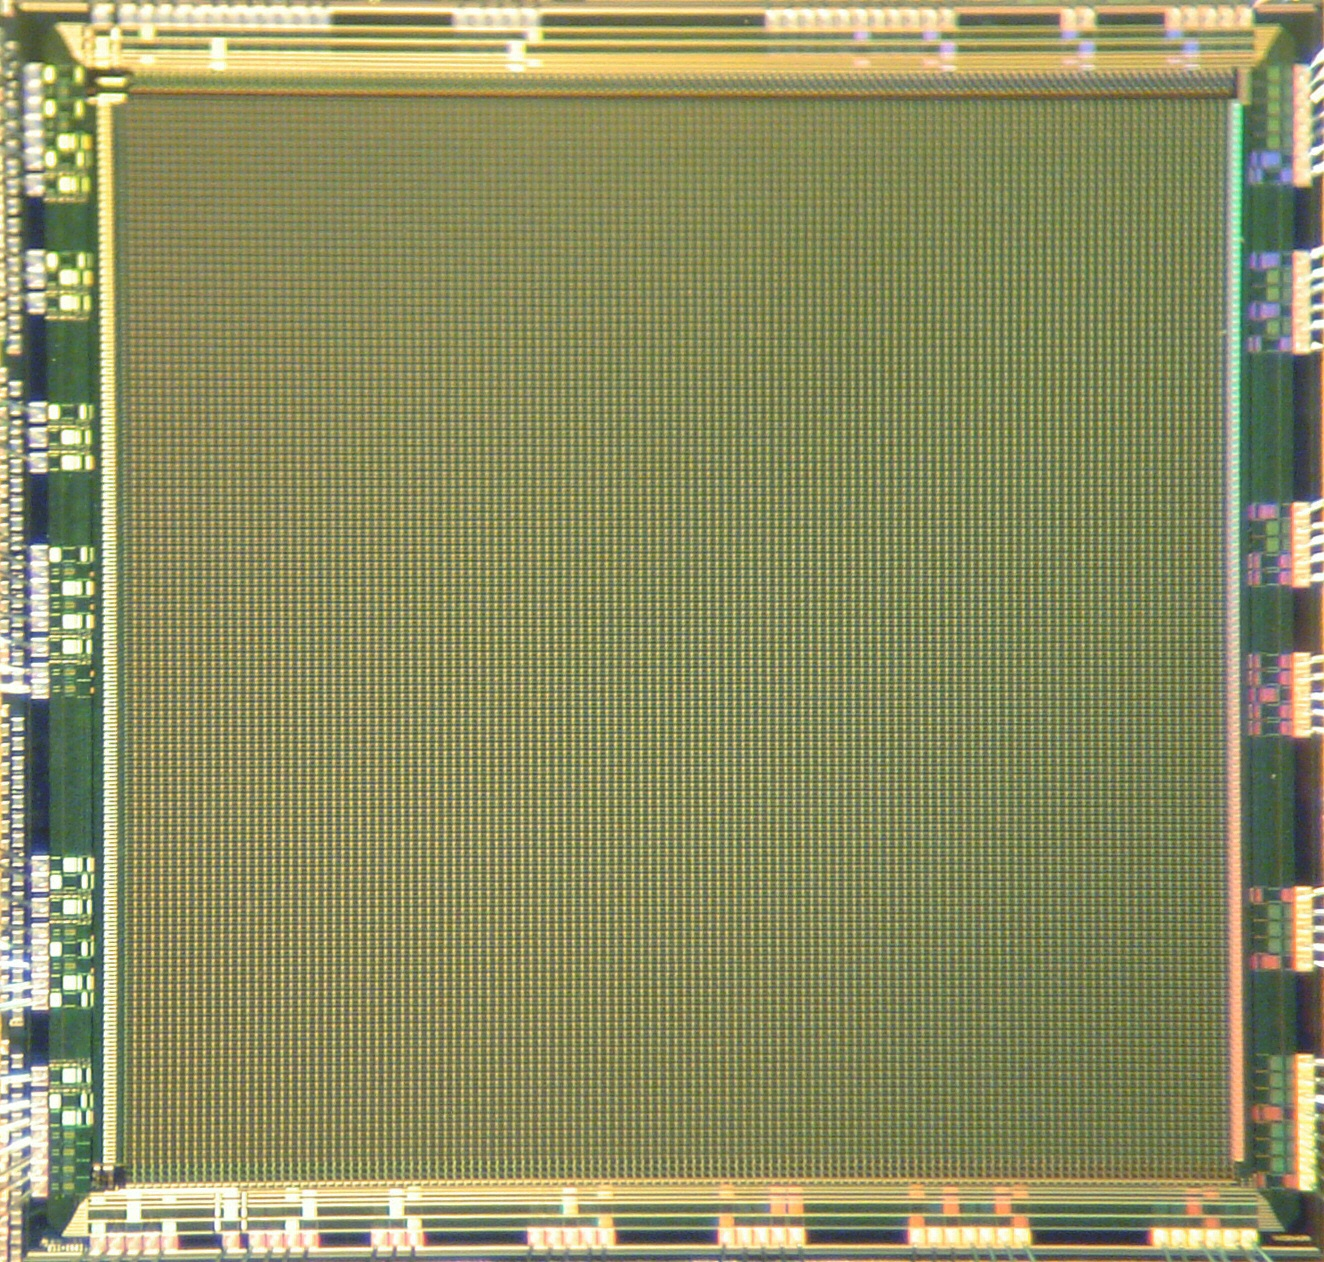
\includegraphics[width=4cm]{scamp3}
%\caption{Le circuit de vision artificielle SCAMP-3 consiste en une grille de $128\times128$ pixels-processeurs\protect\footnotemark.}
%\label{scamp3}
%\end{figure}

%\footnotetext{http://personalpages.manchester.ac.uk/staff/p.dudek/scamp2}

\vspace{-0.5em}
Il existe plusieurs types de polyominos, ceux que nous utiliserons ici sont des ensembles finis de carrés unités connexes par les arêtes dans le plan discret.

\begin{figure}[h]
\centering
\begin{subfigure}[b]{.1\linewidth}
\begin{tikzpicture}[scale=.25, every node/.style={draw, fill=green, rectangle, inner sep=1.25mm}]
\node at (0,0) {};
\node at (1,0) {};
\node at (2,0) {};
\node at (1,1) {};
\end{tikzpicture}
\end{subfigure}
\begin{subfigure}[b]{.1\linewidth}
\begin{tikzpicture}[scale=.25, every node/.style={draw, fill=yellow, rectangle, inner sep=1.25mm}]
\node at (0,0) {};
\node at (0,1) {};
\node at (0,2) {};
\node at (1,0) {};
\end{tikzpicture}
\end{subfigure}
\begin{subfigure}[b]{.1\linewidth}
\begin{tikzpicture}[scale=.25, every node/.style={draw, fill=blue, rectangle, inner sep=1.25mm}]
\node at (1,0) {};
\node at (1,1) {};
\node at (1,2) {};
\node at (0,0) {};
\end{tikzpicture}
\end{subfigure}
\begin{subfigure}[b]{.1\linewidth}
\begin{tikzpicture}[scale=.25, every node/.style={draw, fill=gray, rectangle, inner sep=1.25mm}]
\node at (0,0) {};
\node at (0,1) {};
\node at (1,1) {};
\node at (1,0) {};
\end{tikzpicture}
\end{subfigure}
\begin{subfigure}[b]{.1\linewidth}
\begin{tikzpicture}[scale=.25, every node/.style={draw, fill=purple, rectangle, inner sep=1.25mm}]
\node at (0,0) {};
\node at (1,0) {};
\node at (1,1) {};
\node at (2,1) {};
\end{tikzpicture}
\end{subfigure}
\begin{subfigure}[b]{.1\linewidth}
\begin{tikzpicture}[scale=.25, every node/.style={draw, fill=magenta, rectangle, inner sep=1.25mm}]
\node at (0,1) {};
\node at (1,0) {};
\node at (1,1) {};
\node at (2,0) {};
\end{tikzpicture}
\end{subfigure}
\begin{subfigure}[b]{.1\linewidth}
\begin{tikzpicture}[scale=.25, every node/.style={draw, fill=cyan, rectangle, inner sep=1.25mm}]
\node at (0,0) {};
\node at (1,0) {};
\node at (2,0) {};
\node at (3,0) {};
\end{tikzpicture}
\end{subfigure}

\caption{Quelques polyominos $4$-connexes bien connus}
\end{figure}
\vspace{-1.6em}
L'énumération des polyominos en général est un problème difficile encore ouvert. Malgré cela, plusieurs sous-classes ont été énumérées avec succès en imposant différentes contraintes géométriques aux polyominos. Par exemple, il est bien connu~\cite{pol,stan} que le nombre de polyominos parallélogrammes, dont les lignes et les colonnes se croisant sur la diagonale principale sont contigües, de semi-perimètre $(n+1)$ est le $n$-ième {\em nombre de Catalan} (séquence M1459 sur \cite{OEIS}).

\vspace{-0.3em}
En revanche, le nombre $a_n$ de polyominos simplement $4$-connexe sans trous à $n$ cellules a été calculé jusqu'à $n=56$ \cite{Jen,oeisA001168} et le comportement asymptotique du nombre ces polyominos $\left\{a_n \right\}_{n \geq 0}$ est borné par la relation $\lim_{n\rightarrow \infty} \left\{a_n \right\}^{1/n}=\mu$ où \ $3.90 < \mu < 4.64$~\cite{JenGutt,KlarnerRivest}.

\vspace{-0.3em}
Le lecteur qui désire en savoir plus peut consulter Viennot~\cite{Vi} pour l'énumération exacte de plusieurs classes de polyomino, ainsi que \cite{MBM94,MBM96,MBM98} pour plus de résultats, et \cite{BFRV06} pour l'énumération d'une sous-classe de tuiles parallélogrammes. Plus récemment, l'énumération de certaines familles de polyominos inscrits dans un rectangle a été obtenue dans \cite{GCN10}.

\vspace{-0.3em}
Malgré le fait que ces problèmes aient été largement étudiés, plusieurs questions demeurent ouvertes. Par exemple, on ne connaît pas de formule close pour le nombre de polyominos, et la génération presque exhaustive par ordinateur (en utilisant le lemme de Burnside pour prendre en compte certaines symétries) demeure la seule façon de les compter. Plusieurs algorithmes existent tels ceux de Redelmeier \cite{Red}, un algorithme inductif, et celui Jensen \cite{Jen} plus rapide et basé sur les matrices de transfert \cite{stan}. Ces deux algorithmes sont exponentiels, et celui de Jensen gagne en vitesse au prix d'une consommation exponentielle de mémoire.

%%%% Ce mémoire s'intéresse aux polyominos ainsi qu'à quelques algorithmes s'y rattachant. 
\vspace{-0.3em}
Au chapitre \ref{chapitre-generation}, nous exposerons en détail une autre méthode de génération exhaustive, introduite dans \cite{FGLT}, basée sur la contrainte des polyominos selon leur \emph{périmètre de site}~\cite{MBM03,Sieben08}. Le périmètre de site est le nombre de cellules extérieures à un polyomino qui touchent sa bordure. Cet algorithme s'inspire du jeu de go \footnote{https://fr.wikipedia.org/wiki/Go\_(jeu)} et utilise deux types de pierres, noires et blanches. Le résultat présenté ici a fait l'objet de la publication suivante

\begin{quote}\setstretch{1.0}Fortier, J., Goupil, A., Lortie, J. et Tremblay, J. (2013). Exhaustive generation of
gominoes. Theoretical Computer Science, 502, 76--87.
\end{quote}


\end{introduction}
% !TEX root = memoire.tex
\chapter{Préliminaires}

Dans ce premier chapitre nous définissons les polyominos et nous introduisons quelques concepts de base s'y rattachants.

\section{Les polyominos}

\begin{definition}
Une \emph{cellule} est un carré unitaire $[x,x+1] \times [y,y+1] \subseteq \R^2$. Ses côtés sont appelés \emph{arêtes}.
\end{definition}

\begin{definition*}
Deux cellules sont dites \emph{4-adjacentes} (resp. \emph{8-adjacentes}) si elles partagent au moins une arête (resp. un sommet).
\end{definition*}

Une définition justifiée par le fait qu'une cellule possède un maximum de $4$ ou $8$ voisins selon le type de connexité.

\begin{definition*}
Un ensemble de cellules est \emph{connexe} si toute paire de cellules est reliée par une suite de cellules adjacentes.
\end{definition*}

\begin{figure}[h]
\centering
\begin{tikzpicture}
\squarepath[orange]{(0,1)}{701}
\pas{0.5,1.5}{1.5,0.5};
\pas{1.5,0.5}{2.5,0.5};
\pas{2.5,0.5}{3.5,1.5};
\expandboundingbox
\end{tikzpicture}
\caption[Un chemin]{Un chemin dans un ensemble de cellules $8$-connexe.}
\end{figure}

Nous pouvons maintenant proposer une première définition du polyomino :

\begin{definition}
Un \emph{polyomino} est un ensemble de cellules $4$-connexe.
\end{definition}

\begin{figure}
\begin{subfigure}[b]{.5\linewidth}
\centering
\scalebox{.5}{
\polyomino[blue]{020}

\polyomino[green]{022446} 

\polyomino[red]{000224466}
}
\caption{Des polyominos}
\end{subfigure}
\begin{subfigure}[b]{.5\linewidth}
\centering
\scalebox{.5}{

\begin{tikzpicture}
\squarepath[orange]{(0,0)}{20}
\squarepath[orange]{(1,-1)}{02}
\expandboundingbox
\end{tikzpicture}

\begin{tikzpicture}
\squarepath[violet]{(0,0)}{000022224444666}
\squarepath[violet]{(2,2)}{{}}
\expandboundingbox
\end{tikzpicture}

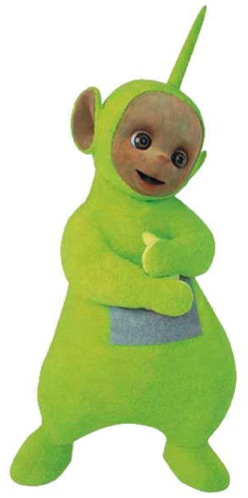
\includegraphics[scale=.3]{dipsy}
}
\caption{Pas des polyominos}
\end{subfigure}
\caption{Exemples de polyominos}\label{fig:exemples-de-polyominos}
\end{figure}

On remarque à la figure \ref{fig:exemples-de-polyominos} que cette définition implique l'existence de polyominos contenant des ``trous''.

\begin{definition}
Soit $P$ un polyomino. Le \emph{contour extérieur} de $P$, $C_e(P)$, est l'ensemble des cellules $4$-connexe à $P$ n'appartenant pas à $P$.
\end{definition}

\begin{definition}
Soit $P$ un polyomino. Son \emph{contour intérieur} $C_i(P)$ est l'intersection entre $P$ et les cellules $4$-connexe à $C_e(P)$.
\end{definition}

Le contour extérieur est connu dans la littérature sous le nom \emph{périmètre de site}. %\cite{Delest:1987aa}.
Pour générer un polyomino, nous générerons son contour défini comme suit \cite{MBM03,Sieben08}  : 

\begin{definition}\label{def:contours}
Le \emph{contour extérieur} d'un polyomino $P$ est l'ensemble $P^+\subseteq\Z^2 \setminus P$ de tous les points $b \in P^+$ qui sont $4$-connexe à au moins un point de $P$. De la même manière, le \emph{contour intérieur} de $P$ est le sous-ensemble $P^-\subseteq P$ de points qui sont $8$-connexes à un point de $\Z^2\setminus P$.
\end{definition}


La figure \ref{fig:contours} illustre le contour intérieur et le contour extérieur d'un polyomino. Il est clair que pour un polyomino donné, ses contours intérieur et extérieur sont uniques.



Quelques propriétés intéressantes :
\renewcommand{\labelitemi}{$\bullet$}
\begin{itemize}
\item $C_e(P) \cap P = \emptyset$
\item $C_i(P) \subseteq P$
\item Pour tout $c \in C_e(P)$, il existe un $t \in P$ tel que $c$ et $t$ sont adjacentes par les côtés.
\end{itemize}




\begin{figure}
\centering
\shorthandoff{:}
\begin{tikzpicture}[scale=0.5]
\draw[color=black!20] (-1.1,-2.1) grid (10.1,8.1);
\squarepath[red]{(0,0)}{000600002022244444444662220000000024444420000};
\savebox{\customwalkbox}{$\circ$}
\custompath{(-0.5,0.5)}{70070000112222233444456445666}
\custompath{(1.5,1.5)}{0070012444444}

\savebox{\customwalkbox}{\large$\bullet$}
\custompath{(0.5,0.5)}{00060000202222242444466444666622200000000}

\squarepath[red]{(11,4.5)}{{}}
\draw (12.5,5) node[right] {Polyomino};

%\draw[tuile] (11,2.5) rectangle ++(1,1);
\draw (11.5,3) node{$\bullet$};
\draw (12.5,3) node[right] {Contour intérieur};

%\draw[draw, black!20] (11,0.5) rectangle ++(1,1);
\draw (11.5,1) node{$\circ$};
\draw (12.5,1) node[right] {Contour extérieur};

\end{tikzpicture}
\caption{Les contours}\label{fig:contours}
\end{figure}


\paragraph{\bf Trous et connexité.}\medskip
On obtient différentes sous-classes de polyominos en ajoutant des contraintes de connectivité. Un polyomino $P$ est \emph{simplement} $4$-connexe (resp. \emph{simplement} $8$-connexe) si son complément $\Z^2 \setminus P$ est également $4$-connexe (resp. $8$-connexe). Par exemple, dans la figure \ref{fig:trous}, le polyomino $P_1$ est simplement $4$-connexe, $P_2$ n'est pas simplement $4$-connexe mais il est simplement $8$-connexe et $P_3$ n'est pas simplement $8$-connexe.
\begin{figure}[h]
\centering
\begin{subfigure}[b]{.2\linewidth}
\centering
\scalebox{.4}{\polyomino[blue]{66020}}
\caption*{$P_1$}
\end{subfigure}
\begin{subfigure}[b]{.2\linewidth}
\centering
\scalebox{.4}{\polyomino[green]{660023}}
\caption*{$P_2$}
\end{subfigure}
\begin{subfigure}[b]{.2\linewidth}
\centering
\scalebox{.4}{\polyomino[red]{66002022446}}
\caption*{$P_3$}
\end{subfigure}
\vspace{-12pt}\caption{Polyominos et trous}
\label{fig:trous}
\end{figure}
\vspace{-12pt}
L'algorithme décrit au chapitre \ref{chapitre-generation} pour la génération exhaustive est assez général pour générer tous ces polyominos. Pour y parvenir, nous devons préciser la notion de \emph{trou}.

\begin{definition}[Trous]\label{def:trous}
Soit $P$ un polyomino. Un \emph{$4$-trou} (resp. \emph{$8$-trou}) de $P$ est un sous-ensemble $4$-connexe (resp. $8$-connexe) maximal et fini de $\Z^2 \setminus P$.
\end{definition}

Ainsi, puisqu'un trou doit être maximal et fini, celui-ci doit être contenu dans un polyomino. Par exemple, dans la figure \ref{fig:trous}, $P_2$ a un $4$-trou, qui dans ce cas est $8$-connexe à une partie infinie de $\Z^2 \setminus P$. Ce n'est donc pas un $8$-trou. Par contre, $P_3$ a un $8$-trou, qui peut aussi être vu comme deux $4$-trous.


\section{Représentations}
Nous avons déjà vu qu'un ensemble de cases connexes par les arêtes est un polyomino.  Il y a plusieurs représentations naturelles qui s'imposent:  graphe de la relation de connectivité, sa réalisation  dans le plan discret $\Z\times\Z$, et  le codage de son contour  par des pas élémentaires. 

\paragraph{\bf Graphe de connexité.}
Parfois l'emplacement précis des cellules n'est pas important, c'est plutôt leur connectivité qui nous intéresse. On construit donc un graphe dont les sommets sont les cellules du polyomino et deux sommets sont reliés par une arête si et seulement si les cellules correspondantes sont $4$-adjacentes.
\begin{figure}[H]
\begin{subfigure}[b]{.5\textwidth}
\centering
\scalebox{0.5}{\polyomino{00204406}}
\end{subfigure}
\begin{subfigure}[b]{.5\textwidth}
\centering
\begin{tikzpicture}[scale=0.5,every node/.style={draw, circle, fill, inner sep=1.5pt}]
\node (a) at (0,0) {};
\node (b) at (1,0) {};
\node (c) at (2,0) {};
\node (d) at (1,1) {};
\node (e) at (2,1) {};
\node (f) at (3,1) {};

\draw[thick] (a) -- (b) -- (c);
\draw[thick] (b) -- (d);
\draw[thick] (c) -- (e);
\draw[thick] (d) -- (e) -- (f);
\end{tikzpicture}
\end{subfigure}
\caption{Un polyomino et son graphe associé}
\end{figure}

\vspace{-24pt}
\paragraph{\bf Sous-ensemble de $\Z^2$.}
Le passage d'un ensemble de tuiles à un ensemble de points à coordonnées entières est naturel. Il suffit de choisir un point canonique sur la tuile, par exemple le plus en bas parmi les plus à gauche. Cette représentation est utilisée entre autre par les physiciens qui nomment ces objets des animaux (\emph{lattice animals} en anglais) \cite{Lubensky79, C3SM52805G} qui surviennent dans des questions reliées à la percolation \cite{KM}.
\begin{figure}[H]
\centering
\shorthandoff{:}
\begin{tikzpicture}[scale=0.5,>=latex,transform shape]
\tuile{0,0};
\tuile{0,1};
\tuile{0,2};
\tuile{0,3};
\tuile{-1,3};
\tuile{0,4};
\tuile{1,0};
\tuile{2,0};
\tuile{0,-1};
\tuile{2,-1};

\begin{scope}[xshift=6.5cm]
\draw[color=black!20] (-2.1, -2.1) grid (3.1,5.1);
\draw[color=black!50, thick, ->] (-1,-2.5) -- (-1,5.5) node [label=above left:$\Z$] {}; 
\draw[color=black!50, thick, ->] (-2.5,3) -- (3.5,3) node [label=below right:$\Z$] {}; 
\point{0,0};
\point{0,1};
\point{0,2};
\point{0,3};
\point{-1,3};
\point{0,4};
\point{1,0};
\point{2,0};
\point{0,-1};
\point{2,-1};
\end{scope}

\end{tikzpicture}
\caption{Un polyomino et son animal}
\end{figure}

Bien que l'utilisation d'éléments de $\Z^2$ donne accès aux outils de la géométrie analytique, le passage du continue au discret reste délicat. Ainsi, même une définition aussi simple que le disque discret $D$ de rayon $r$ centré en $C$ présente certains problèmes
\[
D = \left \{ (x,y) \st {(x-C_x)}^2+{(y-C_y)}^2 \leq r^2, x,y \in \Z\right\}.
\]
Dans \cite{inertia} par exemple, on étudie ces disques et leur comportement lorsque $C$ varie de façon continue dans $\R^2$ (figure \ref{disque-discret}).

\begin{figure}[H]
\centering
\begin{subfigure}{.4\textwidth}
\centering
\begin{tikzpicture}[scale=0.5,transform shape,auto]
\shorthandoff{:}
\draw[black!20] (-2.1,-2.1) grid (2.1,2.1);
\draw[black!50, ->, >=latex] (-2.2, 0) -- (2.2, 0) node[label=below right:$\Z$]{};
\draw[black!50, ->, >=latex] (0,-2.2) -- (0, 2.2) node[label=above left:$\Z$]{};
\fill[blue, opacity=.1] (0.15,0.15) circle (1.5);
\draw[blue!60!black] (0.15,0.15) circle (1.5);
\end{tikzpicture}
\caption{Centré en $(0.15,0.15)$}\label{disque-decentre}
\end{subfigure}
\begin{subfigure}{.4\textwidth}
\centering
\begin{tikzpicture}[scale=0.5,transform shape,auto]
\shorthandoff{:}
\draw[black!20] (-2.1,-2.1) grid (2.1,2.1);
\draw[black!50, ->, >=latex] (-2.2, 0) -- (2.2, 0) node[label=below right:$\Z$]{};
\draw[black!50, ->, >=latex] (0,-2.2) -- (0, 2.2) node[label=above left:$\Z$]{};
\foreach \p in {(1,0),(1,1),(0,1),(-1,1),(-1,0),(0,-1),(1,-1),(0,0)}
  \fill \p circle (3pt);
\end{tikzpicture}
\caption{Discrétisation de \ref{disque-decentre}}
\end{subfigure}

\centering
\begin{subfigure}{.4\textwidth}
\centering
\begin{tikzpicture}[scale=0.5,transform shape,auto]
\shorthandoff{:}
\draw[black!20] (-2.1,-2.1) grid (2.1,2.1);
\draw[black!50, ->, >=latex] (-2.2, 0) -- (2.2, 0) node[label=below right:$\Z$]{};
\draw[black!50, ->, >=latex] (0,-2.2) -- (0, 2.2) node[label=above left:$\Z$]{};
\fill[blue, opacity=.1] (0,0) circle (1.5);
\draw[blue!60!black] (0,0) circle (1.5);
\end{tikzpicture}
\caption{Centré en $(0,0)$}\label{disque-centre}
\end{subfigure}
\begin{subfigure}{.4\textwidth}
\centering
\begin{tikzpicture}[scale=0.5,transform shape,auto]
\shorthandoff{:}
\draw[black!20] (-2.1,-2.1) grid (2.1,2.1);
\draw[black!50, ->, >=latex] (-2.2, 0) -- (2.2, 0) node[label=below right:$\Z$]{};
\draw[black!50, ->, >=latex] (0,-2.2) -- (0, 2.2) node[label=above left:$\Z$]{};
\foreach \p in {(1,0),(1,1),(0,1),(-1,1),(-1,0),(-1,-1),(0,-1),(1,-1),(0,0)}
  \fill \p circle (3pt);
\end{tikzpicture}
\caption{Discrétisation de \ref{disque-centre}}
\end{subfigure}
\caption{Disques de rayon 1.5 et leur équivalent discret.}\label{disque-discret}
\end{figure}


\paragraph{\bf Mot de contour.}

Un \emph{alphabet} est un ensemble fini de symboles. Un \emph{mot} $m$ sur l'alphabet $\mathcal{A}$ est une séquence finie de symboles $a_i \in \mathcal{A}, i \in \N$.
\[
m = a_1 a_1 a_2 \cdots a_{n} 
\]

On note $|m|$ la longueur du mot $m$, et $m_i$ (ou $m[i]$ pour une notation plus près de l'informatique) sa $i^{\rm i\grave{e}me}$ lettre. Le nombre d'occurrences de $\alpha \in \mathcal{A}$ dans $m$ est noté $|m|_\alpha$ et le mot de longueur $0$ est appelé le mot vide qu'on note $\varepsilon$. On remarque que les indices sont entre $1$ et $|m|$ et non entre $0$ et $|m|-1$.

On note $\mathcal{A}^n$ l'ensemble des mots de longueur $n$, et $\mathcal{A}^*$ l'ensemble des mots finis. 

\begin{definition*}
À l'aide de deux mots $a \in \mathcal{A}^m$ et $b \in \mathcal{A}^n$ on obtient par \emph{concaténation}, ou \emph{produit}, le mot $a \cdot b\in \mathcal{A}^{m+n}$, ou simplement $ab$. 
\begin{eqnarray*}
a & = & a_1 a_2 \cdots a_m \\
b & = & b_1 b_2 \cdots b_n \\
ab & = & a_1 a_2 \cdots a_m b_1 b_2 \cdots b_n \\
\end{eqnarray*}
\end{definition*}

%\begin{proposition*}
%$\mathcal{A}^*$ est doté d'une structure de monoïde libre.
%\end{proposition*}

\begin{figure}
\centering
\begin{subfigure}[b]{.25\textwidth}
\centering
\begin{tikzpicture}[scale=.3]
\node[name=O,circle,inner sep=.1cm,fill=black,scale=.4] at (0,0) {};
\node[name=E,draw=none] at (2,0) {$0$};
\node[name=N,draw=none] at (0,2) {$1$};
\node[name=W,draw=none] at (-2,0) {$2$};
\node[name=S,draw=none] at (0,-2) {$3$};
\node[draw=none] at (-3,0) {};
\node[draw=none] at (3,0) {};

\draw[->] (O) to (E);
\draw[->] (O) to (N);
\draw[->] (O) to (W);
\draw[->] (O) to (S);
\end{tikzpicture}
\end{subfigure}
\centering
\begin{subfigure}[b]{.25\textwidth}
\begin{tikzpicture}[scale=.3]
\node[name=O,circle,inner sep=.1cm,fill=black,scale=.4] at (0,0) {};
\node[name=E,draw=none] at (2,0) {$0$};
\node[name=NE,draw=none] at (2,2) {$1$};
\node[name=N,draw=none] at (0,2) {$2$};
\node[name=NW,draw=none] at (-2,2) {$3$};
\node[name=W,draw=none] at (-2,0) {$4$};
\node[name=SW,draw=none] at (-2,-2) {$5$};
\node[name=S,draw=none] at (0,-2) {$6$};
\node[name=SE,draw=none] at (2,-2) {$7$};
\node[draw=none] at (-3,0) {};
\node[draw=none] at (3,0) {};
\draw[->] (O) to (E);
\draw[->] (O) to (N);
\draw[->] (O) to (W);
\draw[->] (O) to (S);
\draw[->] (O) to (NE);
\draw[->] (O) to (NW);
\draw[->] (O) to (SW);
\draw[->] (O) to (SE);
\end{tikzpicture}
\end{subfigure}
\caption{Directions associées à deux alphabets de Freeman}\label{fig:alphabet-freeman}
\end{figure}


En 1961, Herbert Freeman propose de décrire des chemins en utilisant quatre "pas" élémentaires $(\rightarrow,\uparrow,\leftarrow,\downarrow)\simeq (0,1,2,3)$ associés à des vecteurs tel qu'illustré à la figure \ref{fig:alphabet-freeman} \cite{freeman1}. On note cet alphabet $\mathcal{F}$. On code un polyomino sans trou à l'aide de ces lettres en parcourant son bord, chaque lettre correspondant à un pas unitaire sur le chemin. On verra aux sections \ref{subsection:4-trous} et \ref{subsection:8-trous} comment étendre ce codage aux polyominos avec trou.

L'alphabet de virages décrit quant à lui les changements de direction durant le parcours. On peut passer d'un mot $f$ sur l'alphabet de Freeman à un mot $v$ sur l'alphabet de virages en soustrayant les valeurs consécutives:
\[
v_i = f_{i+1} - f_{i} \mod 4 \quad 1 \leq i \le |f|
\]

Pour cette raison on le nomme aussi alphabet des premières différences. On interprète les valeurs $(0,1,2,3)\simeq ($tout droit, gauche, demi-tour, droite$)$. En nous limitant aux mots de contour, qui ne contiennent pas de demi-tour, l'alphabet des premières différences est donc $\{0,1,3\}$.

Un \emph{$4$-chemin} (respectivement \emph{$8$-chemin}) est un chemin qui n'utilise que des pas unité horizontaux et verticaux (respectivement horizontaux, verticaux et diagonaux) . Si ce chemin est fermé et simple, c'est-à-dire que le point d'origine est visité exactement $2$ fois, tandis que tous les autres points sont visités au maximum une fois, alors ce chemin décrit le contour d'un polyomino sans trou.
\begin{figure}[H]
\begin{subfigure}{.33\linewidth}
\centering
\begin{tikzpicture}
\tuile{0,0};
\tuile{1,0};
\end{tikzpicture}
\end{subfigure}
\begin{subfigure}{.33\linewidth}
\centering
\begin{tikzpicture}[>=latex, auto, pas/.style={->, swap, shorten >=2pt}]
\point{0,0};
\draw[pas] (0,0) to node{$0$} (1,0);
\draw[pas] (1,0) to node{$0$} (2,0);
\draw[pas] (2,0) to node{$1$} (2,1);
\draw[pas] (2,1) to node{$2$} (1,1);
\draw[pas] (1,1) to node{$2$} (0,1);
\draw[pas] (0,1) to node{$3$} (0,0);

%\draw[->, swap, bend right] (0,0) to node{0} (1,0) to node{0} (2,0) to node{2} (2,1) to (1,1) to (0,1) to (0,0);

\end{tikzpicture}
\end{subfigure}\begin{subfigure}{.33\linewidth}\centering \ocr{001223} \end{subfigure}

\caption{Un polyomino, son contour et son mot de contour}
\end{figure}


%\begin{preuve}
%\begin{enumerate}
%\item $\forall a,b \in \A^*, ab \in \A^*.$
%\item $\forall a,b,c \in \A^*, ab(c) = a(bc).$
%\item $\forall a \in A^*, a\varepsilon = \varepsilon a = a.$
%\item $\A$ est une base de $\A^*.$
%\end{enumerate}
%\end{preuve}

% !TEX root = memoire.tex
\chapter{Enveloppe externe d'un chemin discret}\label{chapitre-chemins}

Nous présenterons dans ce chapitre un algorithme linéaire pour calculer l'enveloppe extérieure d'un chemin discret décrit par un code de Freeman. Le lien étroit entre un contour et un chemin simple mène à l'utilisation d'une structure d'arbre radix augmenté introduite par \cite{BKP} pour détecter les intersections, qui permet un stockage linéaire des points visités ainsi que leur liens de voisinage dans le plan discret $\Z \times \Z$. Cette structure de données combinée à l'algorithme de la main droite, bien connu pour la résolution de labyrinthe, permet d'obtenir un algorithme linéaire pour calculer l'enveloppe externe. Les résultats de ce chapitre ont été présentés à la conférence internationale DGCI 2014 \cite{BTTW14}.

\begin{figure}[H]
\centering
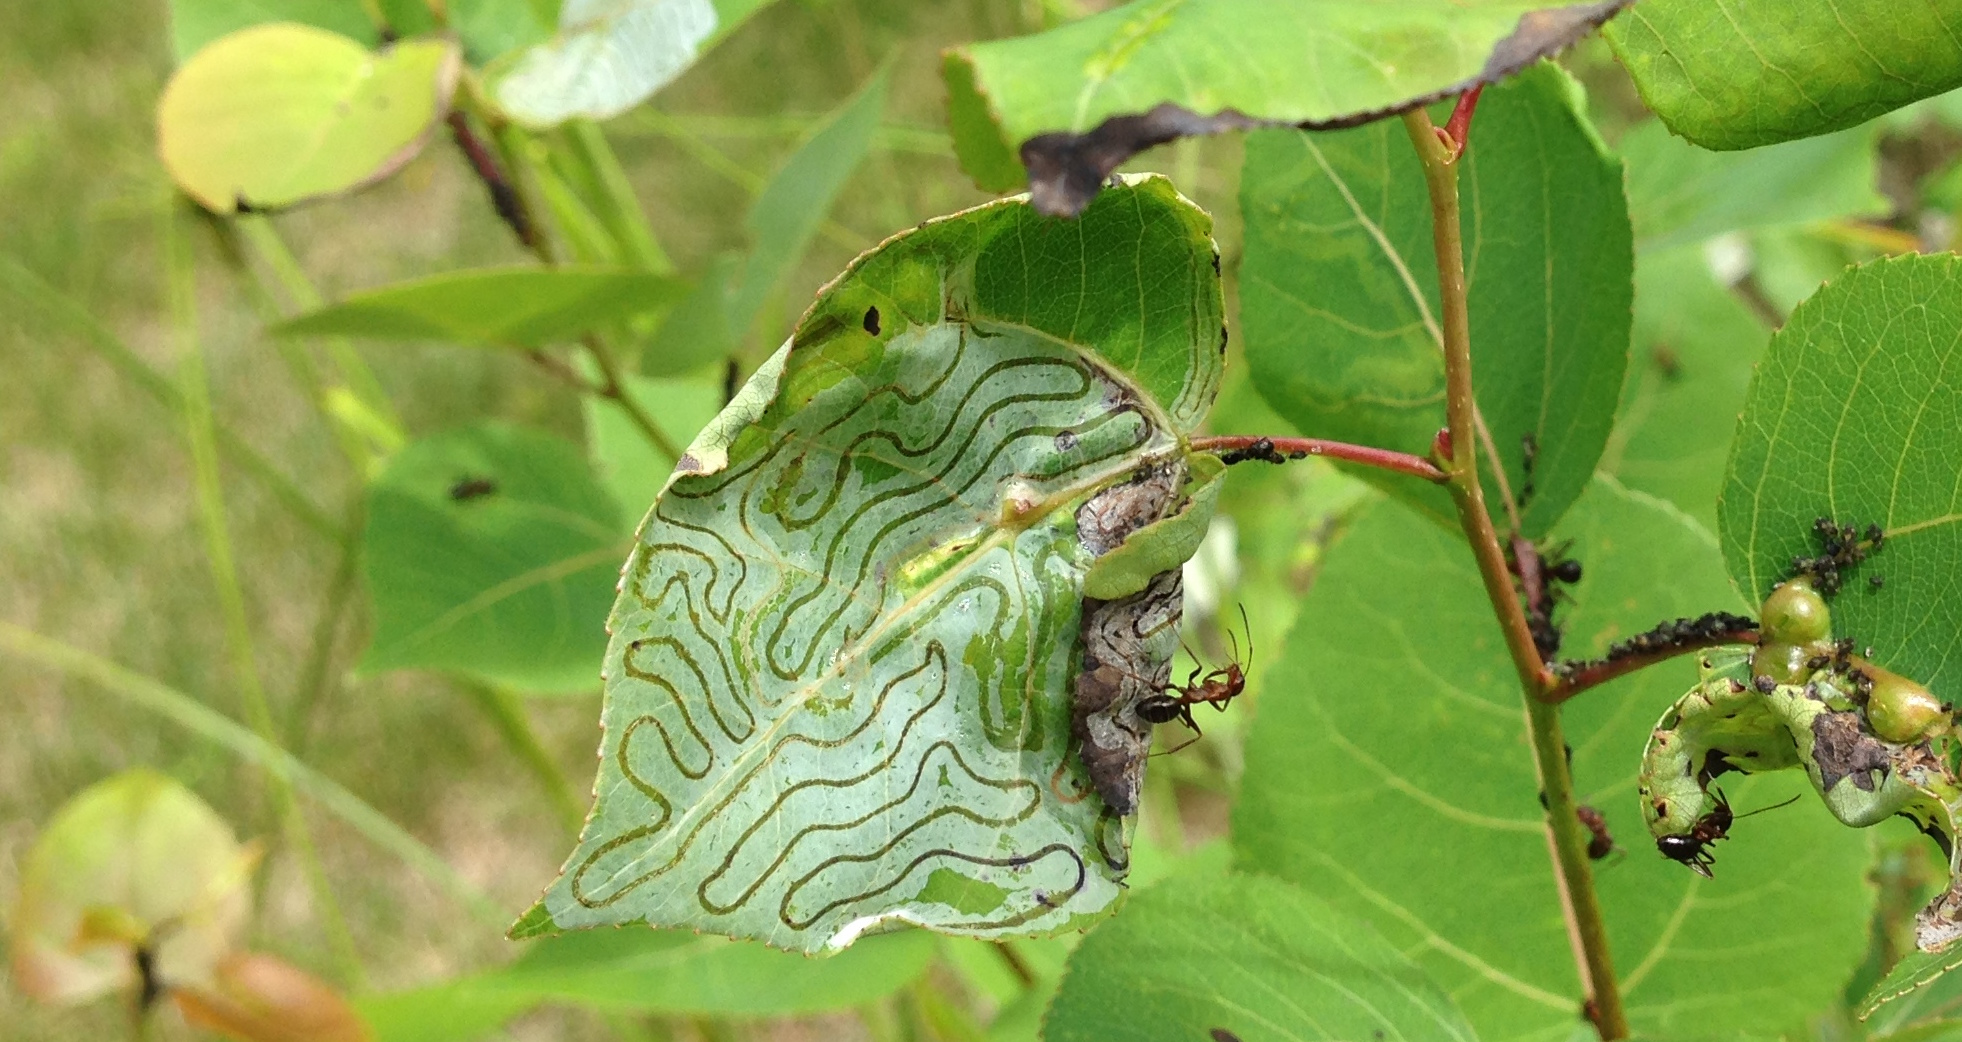
\includegraphics[width=0.8\textwidth]{fourmi}
\caption{L'algorithme glouton de la chenille produit un chemin simple.}
\end{figure}

\section{Les chemins}\label{chemins:preliminaires}


\begin{definition}
L'\emph{ensemble de pas unitaires} est l'ensemble des points de $\Z^2$ accessibles à partir de $(0,0)$ en une seule opération.
\end{definition}

Les pas élémentaires de l'alphabet de Freeman forment un ensemble de pas unitaire.
$$\mathcal{F}=\left\{0,1,2,3\right\} \simeq \left\{(1,0),(0,1),(−1,0),(0,−1)\right\}$$

\begin{definition}
Soit $P$ un ensemble de pas unitaires. Un \emph{chemin} $c=c_0,c_1,...,c_{n-1}$ est une suite de points tels que pour tout $i>0$, il existe au moins un $p\in P$ tel que $c_{i} = c_{i-1} + p$.
\end{definition}

On remarque que $c_0$ est indépendant de $P$. On peut ancrer un chemin n'importe où.

\begin{proposition}
Soit $P=\left\lbrace (1,0),(0,1),(-1,0),(0,-1) \right\rbrace$. Pour tout chemin $C$ à pas unitaires dans $P$ enraciné en $c_0 \in \Z^2$, on a $C \subset \Z^2$.
\end{proposition}
 
\begin{definition}
Un chemin est \emph{discret} lorsque tous ses points sonts dans $\Z^2$.
\end{definition}

On vérifie facilement que si $c_0$ est à coordonnées entières, un chemin est discret.
 
\begin{definition}
Un chemin est \emph{fermé} s'il existe un pas unitaire $p$ tel que $c_0 = c_{n-1}+p$.
\end{definition}

\begin{definition}
Un chemin est \emph{simple} si ses points sont visités exactement une fois. Un chemin simple peut être \emph{fermé} si seul son point d'origine est visité une deuxième fois, au dernier pas.
\end{definition}

Il y a une bijection entre les cellules et $\Z^2$ obtenue en associant $(a,b)\in \Z^2$ au carré unitaire dont le coin inférieur gauche est de coordonnée $(a,b)$. Ainsi, on peut considérer les cellules comme des éléments de $\Z^2$. Par définition, un \emph{ensemble discret} $S$ est un ensemble de cellules, i.e. $S\subset \Z^2$.

Une façon pratique de représenter un ensemble connexe discret sans trous est d'utiliser un mot décrivant son contour. Puisque le contour d'un ensemble discret est un chemin, on utilise le codage de Freeman qui représente efficacement un chemin discret dans $\Z^2$.

\newcommand{\firstdifference}{\ensuremath{\mathbf{\Delta}}}

Il est clair de ces définitions que tout chemin discret $C$ est représenté par un mot $w\in \F^*$ où $\F=\{\ocr{0},\ocr{1},\ocr{2},\ocr{3}\}$ est l'alphabet de Freeman. Il est intéressant de mentioner ici que dans le cas d'un chemin discret fermé, $w$ est unique à permutation circulaire des lettres près. On peut vérifier à l'aide de la figure \ref{fig:2.1} que toute permutation circulaire du mot $w=\ocr{001100322223}$ représente le même chemin, que $w$ est non simple, fermé, et que $$\firstdifference(w)=\ocr{01030330001}$$
code bien les virages de $w$.

\begin{figure}
\begin{subfigure}[b]{.5\textwidth}
\centering
\begin{tikzpicture}[
	l/.style={font=\tiny}, >=latex, auto]
	\draw[help lines, opacity=0.3] (-0.1,-0.1) grid (6.1, 4.1);
	\node[circle, draw, fill, inner sep=1] at (1,1) {};

	\draw[very thick] (1,1) --node[l, swap]{0} ++(1,0)  --node[l, swap]{0} ++(1,0)  --node[l, swap]{1} ++(0,1)  --node[l, swap]{1} ++(0,1)  --node[l, swap]{0} ++(1,0)  --node[l, swap]{0} ++(1,0)  --node[l, swap]{3} ++(0,-1)  --node[l, swap]{2} ++(-1,0)  --node[l, swap]{2} ++(-0.9,0);
	\draw[very thick] (2.9,2)  --node[l,swap]{2} ++(-0.9,0)  --node[l,swap]{2} ++(-1,0) --node[l,swap]{3} ++(0,-1)[->];


\end{tikzpicture}
\caption{$w=\ocr{001100322223};$}\label{fig:2.1a}
\end{subfigure}
\begin{subfigure}[b]{.5\textwidth}
\centering
\begin{tikzpicture}[polyomino/.style={red, very thick, fill=red, fill opacity=0.3}, l/.style={font=\tiny}, >=latex]
	\draw[help lines, opacity=0.3] (-0.1,-0.1) grid (6.1, 4.1);
	%\draw[very thick,->] (0,0) -- (0, 4.3);
	%\draw[very thick,->] (0,0) -- (6.3, 0);
	\node[circle, draw, fill, inner sep=1] at (1,1) {};

	\draw[very thick] (1,1) --++(1,0)  --++(1,0)  --++(0,1)  --++(0,1)  --++(1,0)  --++(1,0)  --++(0,-1)  --++(-1,0)  --++(-0.9,0);
	\draw[very thick] (2.9,2)  --++(-0.9,0)  --++(-1,0) --++(0,-1)[->];

	\draw[cyan] (1.9,0.9) -- ++(0.3, 0)[->];
	\draw[cyan] (2.9,0.9) -- ++(0.1, 0) arc (-90:0:0.1) -- ++(0,0.2)[->];
	\draw[cyan] (3.1,1.9) -- ++(0, 0.3)[->];
	\draw[cyan] (3.1,2.7) -- ++(0, 0.1) arc (180:90:0.1) -- ++(0.2,0)[->];

	\draw[cyan] (3.9,2.9) -- ++(0.3, 0)[->];
	\draw[cyan] (4.7,2.9) -- ++(0.1, 0) arc (90:0:0.1) -- ++(0,-0.2)[->];
	\draw[cyan] (4.9,2.3) -- ++(0,-0.1) arc (0:-90:0.1) -- ++(-0.2,0)[->];
	\draw[cyan] (4.1,2.1) -- ++(-0.3,0)[->];
	\draw[cyan] (3.05,2.15) -- ++(-0.3,0)[->];
	\draw[cyan] (2.1,2.1) -- ++(-0.3,0)[->];
	\draw[cyan] (1.1,2.1) -- ++(-0.1,0) arc (90:180:0.1) -- ++(0,-0.2)[->];
	
	\node[l] at (2,0.75) {0};
	\node[l] at (3.15,0.85) {1};
	\node[l] at (3.25,2.15) {0};
	\node[l] at (3.25,2.75) {3};
	\node[l] at (4,2.75) {0};
	\node[l] at (4.75,2.75) {3};
	\node[l] at (4.75,2.25) {3};
	\node[l] at (4,2.25) {0};
	\node[l] at (2.75,2.25) {0};
	\node[l] at (2,2.25) {0};
	\node[l] at (0.85,2.15) {1};
\end{tikzpicture}
\caption{$\firstdifference(w)=\ocr{01030330001};$}\label{fig:2.1b}
\end{subfigure}
\caption{Deux codages du même chemin}\label{fig:2.1}
\end{figure}

Tout chemin est contenu dans un plus petit rectangle, appelé la \emph{boîte englobante} (ou \emph{bounding box} en anglais). On définit $W$ comme étant le point le plus bas parmi les points les plus à gauche sur cette boîte tel qu'illustré à la figure \ref{fig:point-W}. On peut facilement obtenir $W$ en temps linéaire en lisant le mot une première fois en conservant les extremums.


\begin{figure}
\begin{subfigure}[b]{.5\linewidth}
\centering
\shorthandoff{:}
\begin{tikzpicture}[>=latex, scale=0.5]
	\draw[help lines, opacity=0.3] (-0.1,-0.1) grid (7.1, 7.1);
	\simplepath[->, very thick]{(3,6)}{6446660246000600224};
	\draw[very thick, opacity=0.3] (1,1) rectangle (6,6);
	\node[circle, draw, fill, inner sep=1, label=below left:{$W$}] at (1,2) {};
\end{tikzpicture}
\caption{}\label{fig:point-Wa}
\end{subfigure}
\begin{subfigure}[b]{.5\linewidth}
\centering
\shorthandoff{:}
\begin{tikzpicture}[>=latex, scale=0.5]
	\squarepath{(1,2)}{06200244202060};
	\draw[help lines, opacity=0.3] (-0.1,-0.1) grid (7.1, 7.1);
	\draw[very thick, opacity=0.3] (1,1) rectangle (6,6);
	\node[circle, draw, fill, inner sep=1, label=below left:{$W$}] at (1,2) {};
	\node[circle, draw, fill, inner sep=1, label=below right:{$S$}] at (3,1) {};
	\node[circle, draw, fill, inner sep=1, label=above right:{$E$}] at (6,5) {};
	\node[circle, draw, fill, inner sep=1, label=above left:{$N$}] at (3,6) {};
\end{tikzpicture}
\caption{}\label{fig:point-Wb}
\end{subfigure}
\caption{Boîte englobante et factorisation standard}\label{fig:point-W}
\end{figure}

On termine cette section avec un bref rappel de topologie des graphes (voir \cite{gross87} pour un traitement plus complet du sujet). Soit $P$ un chemin discret (i.e. une suite de points entiers) codés par le mot $w$. L'image de $P$ comme un sous-ensemble de $\R^2$ est notée $G_P$ tandis que le graphe de l'image plongé dans le dans le plan $\R^2$ est notée $\mathcal{G}(P)$.

Le \emph{plongement} d'un graphe $G$ sur une surface $S$ fait correspondre des points de $S$ aux sommets de $G$ et des \emph{arcs simples} (images homéomorphiques de $[0,1]$) aux arêtes de $G$ de telle façon à ce que :

\begin{itemize}
\item Les extrémités de l'arc associé à l'arête $e$ sont les points associés aux sommets aux extrémités de $e$.
\item Aucun arc ne contient de points associés à un autre sommet.
\item Deux arcs ne se croisent pas en un point contenu dans l'un des deux arcs.
\end{itemize}

Intuitivement, cela signifie que les arcs ne se croisent pas et ne passent pas par un sommet.

Dans le cas du graphe associé au chemin discret $P$, un tel plongement est complètement déterminé en associant un ordre cyclique aux arêtes autour de chaque sommet de la façon suivante : d'abord on fixe une orientation en chaque point (par exemple anti-horaire). Ensuite, pour chaque sommet $v$ dans $G_P$, on définit la permutation cyclique sur les arêtes entrantes de $v$. Ceci définit un schéma de rotation sur $G_P$. On peut montrer qu'un tel schéma de rotation est équivalent à un plongement orienté de $G_P$ sur une surface. Par exemple, la figure \ref{fig:plongement} illustre le chemin $P$ codé par $w=\ocr{001322}$, son graphe $G_P$ et son plongement anti-horaire $\mathcal{G}_P$ dans $\R^2$.

\begin{figure}
\centering
\begin{subfigure}[b]{.3\linewidth}
\centering
\shorthandoff{:}
\begin{tikzpicture}[>=latex, scale=1]
	\node[fill, circle, inner sep=1.5] at (1,2) {};
	\draw[help lines, opacity=0.3] (-0.1,-0.1) grid (4.1, 4.1);
	\simplepath[->, very thick]{(2,2)}{02466};
	\node[fill=white, inner sep=0.2em] at (2,2) {};
	\simplepath[very thick]{(1,2)}{00};
\end{tikzpicture}
\caption{}
\end{subfigure}
\begin{subfigure}[b]{.3\linewidth}
\centering
\shorthandoff{:}
\begin{tikzpicture}[>=latex, scale=1,
	sommet/.style={fill, circle, inner sep=1.5}]
	\node[fill=white, inner sep=0.5em] at (2,2) {};
	\simplepath[very thick]{(1,2)}{002466};
	\node[sommet, label=west:{A}] at (1,2) {};
	\node[sommet, label=north west:{E}] at (2,2) {};
	\node[sommet, label=south east:{D}] at (3,2) {};
	\node[sommet, label=north east:{C}] at (3,3) {};
	\node[sommet, label=north west:{B}] at (2,3) {};
	\node[sommet, label=south:{F}] at (2,1) {};
\end{tikzpicture}
\caption{}
\end{subfigure}
\begin{subfigure}[b]{.3\linewidth}
\centering
\renewcommand{\arraystretch}{0.6}
\begin{tabular}{rcl}
A & : & E\\
B & : & C E\\
C & : & B D\\
D & : & C E\\
E & : & A F D B\\
F & : & E\\
\end{tabular}
\caption{}
\end{subfigure}
\caption{(a) Le graphe $G_P$ codé par le mot $w=\ocr{001233}$; (b) Le plongement anti-horaire de $\mathcal{G}(P)$ dans $\R^2$; (c) Le schéma de rotation de $\mathcal{G}(P)$.}\label{fig:plongement}
\end{figure}

Puisque par définition un plongement de $P$ est planaire, la surface sur laquelle $P$ est plongée se trouve partagée en un certain nombre de régions mutuellement exclusives délimitées par $\mathcal{G}(P)$. On nomme ces régions \emph{faces} et dans le cas d'une surface infinie comme $\R^2$, toutes les faces sont de taille finie sauf une. Cette face non-bornée est la \emph{face externe} de $\mathcal{G}(P)$.

\section{Enveloppes externes et convexes}

\newcommand{\hull}[1]{\text{Hull}(#1)}

On rappelle qu'en topologie, étant donné un ensemble $S$, le bord $\partial S$ est l'ensemble des points dans l'adhérence de $S$ qui ne sont pas à l'intérieur de $S$. L'\emph{enveloppe externe} de $S$, notée $\hull{S}$, est le bord de l'intersection de tous les ensembles discrets sans trous contenant $S$, i.e. le chemin simple suivant le contour de $S$. La définition \ref{def:outer-hull} étend la notion d'enveloppe externe à tout chemin discret.

\begin{definition}\label{def:outer-hull}
Soit $P$ un chemin discret. Alors, l'enveloppe externe de $P$, notée $\hull{P}$ est la face externe de $\mathcal{G}(P)$, le plongement de $P$.
\end{definition}

On note que la définition \ref{def:outer-hull} utilise le plongement de $P$ plutôt qu'un ensemble discret pour décrire l'enveloppe externe. Ce choix permet de décrire l'enveloppe d'un chemin discret (i.e. un ensemble Euclidien d'aire $0$). Par exemple, la figure \ref{chemin-et-enveloppe-externe} illustre l'enveloppe externe du chemin $w=021$.  On remarque aussi qu'en utilisant la définition \ref{def:outer-hull}, le bord d'un chemin est codé par un mot fermé. e.g. l'enveloppe externe du chemin codé par $0$ est codé par $02$. Ainsi, la définition \ref{def:outer-hull} offre une généralisation adéquate de l'enveloppe externe aux chemins discrets quelconques. En effet, si $P$ code le bord d'un ensemble discret sans trou $S$, alors $P$ est simple et fermé par définition. Donc $P=\hull{P}$ et donc puisque $\hull{S}$ est le bord $\partial S$ de $S$ par définition, on a
\begin{equation}
\hull{S} = \partial S = P = \hull{P}\text{.}
\end{equation}

\begin{figure}
\centering
\begin{subfigure}[b]{.3\textwidth}
\centering
\shorthandoff{:}
\begin{tikzpicture}[>=latex, scale=1, auto]
	\draw[help lines, opacity=0.3] (-0.1,-0.1) grid (3.1, 3.1);
	\node[fill, circle, inner sep=1.5] at (1,1) {};
	\simplepath[->, very thick]{(1,1)}{042};
	\path (1,1) -- node[swap]{\tiny 0} (2,1) -- node[swap]{\tiny 2} (1,1) -- node[swap]{\tiny 1} (1,2);
\end{tikzpicture}
\end{subfigure}
\begin{subfigure}[b]{.3\textwidth}
\centering
\shorthandoff{:}
\begin{tikzpicture}[>=latex, scale=1, auto]
	\draw[help lines, opacity=0.3] (-0.1,-0.1) grid (3.1, 3.1);
	\node[fill, circle, inner sep=1.5] at (1,1) {};
	\simplepath[->, very thick]{(1,1)}{042};
	\draw[rounded corners=2.8pt, ->] (1.9, 0.9) -- (2.1, 0.9) -- node[swap, midway]{\tiny $2$} (2.1,1.1) -- (1.8, 1.1);
	\draw[rounded corners=2.8pt, ->] (1.3, 1.1) -- (1.1, 1.1) -- node[swap]{\tiny $3$} (1.1, 1.4);
\end{tikzpicture}
\end{subfigure}
\begin{subfigure}[b]{.3\textwidth}
\centering
\end{subfigure}
\begin{subfigure}[b]{.3\textwidth}
\centering
\shorthandoff{:}
\begin{tikzpicture}[>=latex, scale=1, auto]
	\draw[help lines, opacity=0.3] (-0.1,-0.1) grid (3.1, 3.1);
	\node[fill, circle, inner sep=1.5] at (1,1) {};
	\simplepath[->, very thick]{(1,1)}{042};
	\draw[rounded corners=2.8pt, ->] (1.1, 0.9) --node[swap, midway]{\tiny $0$} (1.9, 0.9) -- (2.1, 0.9) -- (2.1,1.1) -- node[swap, midway]{\tiny $2$} (1.1, 1.1) --node[swap, midway]{\tiny $1$} (1.1, 2.1) -- (0.9, 2.1) --node[swap, midway]{\tiny $3$} (0.9, 1.1);
\end{tikzpicture}
\end{subfigure}
\begin{subfigure}[b]{.3\textwidth}
\centering
\end{subfigure}
\caption{Chemin \ocr{021} et son enveloppe externe}\label{chemin-et-enveloppe-externe}
\end{figure}

Puisqu'il y a une bijection entre les chemins discrets dans $\Z^2$ et les mots sur $\F$, on identifie $P$ à son mot $w$ et on écrit $\hull{w}$ plutôt que $\hull{P}$.

Pour finir, on rappelle certaines notions de base concernant la convexité digitale tout en référant le lecteur intéressé à \cite{blpr09,thesexavier} pour une couverture plus complète du sujet. Soit $S$ un ensemble discret $8$-connexe. $S$ est \emph{digitalement convexe} s'il s'agit de la digitalisation de Gauss d'un sous-ensemble convexe $R$ de $\R^2$, i.e. $S=\conv{R}\cap \Z^2$. L'\emph{enveloppe convexe de $S$}, notée $\conv{S}$ est l'intersection de tous les ensembles convexes contenant $S$. Dans le cas d'un chemin simple $w$, $\conv{w}$ est donnée par la factorisation de Spitzer de $w$ (voir \cite{spitzer56,blpr09}). Étant donné $w=w_1w_2\cdots w_n \in \{0,1\}^*$, on calcule le segment $NW$ de la factorisation de la manière suivante: commencer avec la liste $(b_1,b_2,\dots,b_n)=(w_1,w_2,\dots,w_n)$. Si la pente $\rho(b_i)=|b_i|_1/|b_i|_0$ de $b_i$ est strictement plus petite que celle de $b_{i+1}$ pour un $i$, alors
\[
(b_1,b_2,\dots,b_k)=(b_1,\dots,b_{i-1},b_i b_{i+1},b_{i+2},\dots,b_k)\text{.}
\]

En répétant le processus jusqu'à ce qu'il soit impossible de concaténer deux autres $b_i$, on obtient la factorisation de Spitzer de $w$. Les parties $NE$, $SE$ et $SW$ de la factorisation sont obtenues par rotation.

\section{Algorithme}

Soit $w\in\F^*$ un chemin discret et $G_w$ sa représentation en graphe. Remarquons que l'application $g:w\rightarrow G_w$ n'est pas bijective puisqu'elle n'est pas injective (par exemple, $u=0$ et $v=02$ admettent le même graphe.). Nous avons vu à la section \ref{chemins:preliminaires} que le plongement $\mathcal{G}(w)$ de $G_w$ dans $\R^2$ donne lieu à un schéma de rotation si l'on fixe une orientation. Nous utilisons ce plongement pour calculer l'enveloppe externe de $w$ (i.e. la face externe de $\mathcal{G}(w)$): on fixe l'orientation $\mathcal{O}$ sur la surface $\R^2$ et on choisit le sommet le plus en bas parmis les plus à gauche, $W$, comme point de départ. Soit $e_0=(W,v)$ un arc allant du sommet $W$ vers le sommet $v$ dans $\mathcal{G}(w)$. Par le choix de $W$, $e_0$ est une arête de la face externe de $\mathcal{G}(w)$. Par récurrence, soit $e_i=(u,v)$ un arc du sommet $u$ vers le sommet $v$ dans $\mathcal{G}(w)$ tel que $e_i$ est une arête de la face externe du plongement $\mathcal{G}(w)$ et tel que $e_i$ suis l'orientation fixée par $\mathcal{O}$. Ensuite, calculer $e_{i+1}=(v,\sigma_v(u))$ où $\sigma_v$ est la permutation cyclique associée à $v$ dans $\mathcal{G}(w)$. Alors $e_{i+1}$ est aussi une arête de la face externe. En choisissant $\mathcal{O}$ anti-horaire, on peut répéter ce processus pour obtenir la face externe de $\mathcal{G}(w)$.

Par exemple, en utilisant le schéma de rotation défini pour $w=\ocr{001233}$ à la figure \ref{fig:plongement}c et en commençant avec l'arc $(A,E)$, on obtient la séquence d'arcs
\[
(A,E), (E,F), (F,E), (E,D), (D,C), (C,B), (B,E), (E,A)
\]
qui correspond à l'enveloppe externe de $w$ (voir figure \ref{fig:sequence-arcs}).

\begin{figure}
\begin{subfigure}[b]{.3\linewidth}
\centering
\shorthandoff{:}
\begin{tikzpicture}[>=latex, scale=1,
	sommet/.style={fill, circle, inner sep=1.5}]
	\node[sommet, label=west:{A}] (A) at (1,2) {};
	\node[sommet, label=north west:{E}] (E) at (2,2) {};
	\node[sommet, label=south east:{D}] (D) at (3,2) {};
	\node[sommet, label=north east:{C}] (C) at (3,3) {};
	\node[sommet, label=north west:{B}] (B) at (2,3) {};
	\node[sommet, label=south:{F}] (F) at (2,1) {};
	
	\path (A) edge[->, bend right] (E);
	\path (E) edge[->, bend right] (F);
	\path (F) edge[->, bend right] (E);
	\path (E) edge[->] (D);
	\path (D) edge[->] (C);
	\path (C) edge[->] (B);
	\path (B) edge[->] (E);
	\path (E) edge[->, bend right] (A);
	
\end{tikzpicture}
\caption{}
\end{subfigure}
\begin{subfigure}[b]{.3\linewidth}
\centering
\shorthandoff{:}
\def\centerarc[#1](#2)(#3:#4:#5){ \draw[#1] ($(#2)+({#5*cos(#3)},{#5*sin(#3)})$) arc (#3:#4:#5); }
\begin{tikzpicture}[>=latex, scale=1, auto, swap,
	s/.style={fill, circle, inner sep=1.5}]
	\draw (0,1) node[s, label=left:{$u$}]{} -- (1,1) node[s, label=above left:{$v$}]{}-- (2,1) node[s, label=right:{$\sigma^2_v(u)$}]{};
	\draw (1,0) node[s, label=below:{$\sigma_v(u)$}]{} -- (1,2) node[s, label=above:{$\sigma^3_v(u)$}]{};
	\draw[red, rounded corners=2.8pt, ->] (0.1, 0.8) -- (0.8, 0.8) -- (0.8, 0.1);
	\draw[red,domain=135:415, xshift=1cm, yshift=1cm, ->] plot ({0.2*cos(\x)}, {0.2*sin(\x)});\end{tikzpicture}
\caption{}\label{sigma-u-v}
\end{subfigure}
\begin{subfigure}[b]{.3\linewidth}
\centering
\shorthandoff{:}
\begin{tikzpicture}[>=latex, scale=1, auto, swap]
	\node[fill, circle, inner sep=1.5] at (1,2) {};
	\draw[help lines, opacity=0.3] (-0.1,-0.1) grid (4.1, 4.1);
	\simplepath[->, very thick]{(2,2)}{02466};
	\node[fill=white, inner sep=0.2em] at (2,2) {};
	\simplepath[very thick]{(1,2)}{00};
	\draw[red, rounded corners=2.8pt, ->]  (1.1, 1.9) -- node{\tiny $0$} (1.9, 1.9) -- node{\tiny $3$} (1.9, 0.9) -- (2.1, 0.9) -- node{\tiny $1$} (2.1, 1.9) -- node{\tiny $0$} (3.1, 1.9) -- node{\tiny $1$} (3.1, 2.9) -- (3.1, 3.1) -- node{\tiny $2$} (1.9, 3.1) -- node{\tiny $3$} (1.9, 2.1) -- node{\tiny $2$} (1.1, 2.1);
\end{tikzpicture}
\caption{}
\end{subfigure}
\caption{Orientation du parcours de $\mathcal{G}(w)$}\label{fig:sequence-arcs}
\end{figure}

La justesse de la méthode découle de la «~règle de la main droite~» ou de «~l'algorithme du mur~» pour traverser un labyrinthe. En effet, étant donné l'arc $(u,v)$, prendre l'arc adjacent $(v,\sigma_v(u))$ revient à «~tourner à droite~» au sommet $v$ (voir figure \ref{sigma-u-v}). Le principe sous-jacent étant donc de commencer sur un point de l'enveloppe externe et rester dessus lors du parcours en prenant systématiquement à droite à chaque intersection, en terminant lors du retour au point de départ. Ceci garantit que le parcours est précisément l'enveloppe externe de $w$.

Pour implémenter efficacement cette méthode, plusieurs problèmes doivent être résolus. Premièrement, tel qu'indiqué plus haut, le parcours doit commencer sur un point de l'enveloppe externe sinon le résultat pourrait ne pas décrire l'objet voulu. On choisit donc le point $W$ associé au mot de contour $w$ comme point de départ.

Deuxièmement, lorsqu'un parcours repasse par $W$ on soit s'assurer que l'algorithme ne termine pas prématurément (le cas le plus simple étant codé par $w=\ocr{021}$, voir la figure \ref{chemin-et-enveloppe-externe}). Une solution simple consiste à construire une liste des voisins de $W$ dans le chemin $P$, et de les retirer lorsqu'ils sont visités. Cette liste contient au plus deux éléments puisqu'aucun sommet de $P$ ne peut se trouver à gauche ou en bas de $W$.

Le dernier problème à résoudre est la détection des intersections. Nous présenterons trois solutions solutions possibles avec des caractéristiques différentes. On cherche une fonction $f(x,y)\rightarrow \{1,0\}$ qui nous indique si l'emplacement $(x,y)$ a déjà été visité.

Première approche, l'adressage direct. Pour conserver la trace d'un chemin de longueur $n$ dans $\Z^2$, on  alloue immédiatement la mémoire pour l'ensemble de positions possibles dans un bloc contigu. On peut ainsi directement calculer l'emplacement de n'importe quelle position visitée. Un tableau $2n \times 2n$ contiendra toutes les positions atteignables par un chemin de longeur $n$ enraciné en $(n,n)$. Dans une telle structure de données, l'accès à une position spécifique se fait en temps constant. Par contre les besoins en mémoire sont  de l'ordre de $\O(n^2)$.

Deuxième approche, le tri. On ajoute chaque nouvelle position visitée à une liste triée. Plusieurs structures de données classiques se prêtent bien à cet usage comme les arbres rouge noir, les arbres B et les arbres AVL par exemple. Pour toutes ces structures de données bien connues, la consommation de mémoire est d'ordre $\O(n)$ et une opération de recherche ou d'insertion est d'ordre $\O(\log(n))$.

\newcommand{\voisin}{\text{\scshape voisin}\xspace}
\newcommand{\enfant}{\text{\scshape enfant}\xspace}
\newcommand{\pere}{\text{\scshape pere}\xspace}
\newcommand{\parcours}{\text{\scshape parcours}\xspace}
\newcommand{\HULL}{\text{\scshape hull}\xspace}

\newcommand{\Nodes}{\mathcal{N}}
\newcommand{\Node}[1]{\fbox{\vphantom{(}#1}}


Troisième approche, l'arbre radix augmenté \cite{BKP}. Soit $G=(\Nodes,E,V)$ un graphe où :
\setlist[description]{font=\normalfont}
\begin{description}
\item[$\Nodes$] Les sommets du graphe, on dira les noeuds, associés aux points de $\Z^2$.
\item[E] Les arêtes du graphe associées à la fonction \enfant.
\item[V] Les arêtes du graphe associées à la fonction \voisin.
\end{description}
On profite du fait que chaque accès est adjacent au précédent. Un noeud $N\in \mathcal{N}$ est défini par le quintuplet $N=(C, E, V, P, \Sigma)$ où $C\in \Z^2$ est la coordonnée cartésienne de ce noeud, $E=(E_0, E_1, E_2, E_3)$ où $E_i\in \mathcal{N}$ sont les quatre enfants, $V=(V_0,V_1,V_2,V_3)$ où $V_i\in{\mathcal{N}}$ sont les voisins, $P\in{\mathcal{N}}$ est le père et $\Sigma\in{\N}$ un compteur du nombre de fois où $N$ est visité. De plus, on permettra d'étiqueter les $V_i$ pour reconnaître un voisin \emph{explicite}, spécifié par le chemin parcouru, ou \emph{implicite}, ajouté par l'algorithme pour accélérer les calculs.

On notera le noeud du point $p$ à l'aide d'une boîte \Node{$p$} et on utilisera la forme \Node{$(x,y)$} pour le noeud de coordonnée $(x,y)$. 

Tout d'abord on considère un arbre contenant les points du plan, construit d'après la fonction $e:\Nodes \rightarrow \Nodes^4$ qui permet de passer d'un noeud à ses 4 enfants:
\begin{equation}
e\left(\Node{$(x,y)$}\right) = \left ( \Node{$(2x,2y)$},\Node{$(2x+1,2y)$},\Node{$(2x+1,2y+1)$},\Node{$(2x,2y+1)$}\right )\text{.}
\end{equation}

On définit la fonction $\text{\scshape enfant}$ comme une restriction de $e$ à l'enfant auquel on souhaite accéder : $$\text{\scshape enfant} : \Nodes \times \Z^2 \rightarrow \Nodes $$ où $\text{\scshape enfant}\left(\Node{$A$}, (x,y)\right) = \Node{$(x,y)$}$ est définie si et seulement si $\Node{$(x,y)$}$ est bel et bien un enfant de $\Node{$A$}$.

On remarque que les coordonnées des enfants sont obtenues en ajoutant $1$ ou $0$ à la représentation binaire des coordonnées du parent tel qu'illustré à la figure \ref{fig:arbre-radix-binaire}.

\begin{figure}
\begin{tikzpicture}[grow=right, sibling distance=2em,
					level distance=4cm]]

\node{(0,0)} 
	child {node {(0,1)}
	}
	child {node {(1,1)}
	}
	child {node {(1,0)}
		child {node {(2,0)}
		}
		child {node {(3,0)}
		}
		child {node {(3,1)}
		}
		child {node {(2,1)}
			child {node {(4,2)}}
			child {node {(5,2)}}
			child {node {(5,3)}}
			child {node {(4,3)}}
		}
	}
;
\end{tikzpicture}

\begin{tikzpicture}[grow=right, sibling distance=2em,
					level distance=4cm]]

\node{(0,0)} 
	child {node {(00,01)}
	}
	child {node {(01,01)}
	}
	child {node {(01,00)}
		child {node {(010,000)}
		}
		child {node {(011,000)}
		}
		child {node {(011,001)}
		}
		child {node {(010,001)}
			child {node {(0100,0010)}}
			child {node {(0101,0010)}}
			child {node {(0101,0011)}}
			child {node {(0100,0011)}}
		}
	}
;
\end{tikzpicture}
\caption{Arbre radix et sa représentation binaire.}\label{fig:arbre-radix-binaire}
\end{figure}

La fonction inverse $$\pere: \Nodes \rightarrow \Nodes$$ permet de passer d'un noeud à son père. On peut aussi calculer directement les coordonnées du père:
\begin{equation}
f(x,y) = \left(\floor*{\frac{x}{2}}, \floor*{\frac{y}{2}}\right)
\end{equation} 
Le fait de connaître les coordonnées du père d'un point sans avoir de référence au noeud de ce point ou à celui de son père est crucial au fonctionnement de l'algorithme. 

\begin{figure}
\begin{tikzpicture}[grow=right, 
					level 1/.style={sibling distance=20em},
					level 2/.style={sibling distance=4.5em},
					level 3/.style={sibling distance=1em, font=\relsize{-2}}, 
					level distance=4cm]]

\node{(0,0)} 
	child {node {(0,1)}
		child {node {(0,2)}
			child {node {(0,4)}}
			child {node {(1,4)}}
			child {node {(1,5)}}
			child {node {(0,5)}}
		}
		child {node {(1,2)}
			child {node {(2,4)}}
			child {node {(3,4)}}
			child {node {(3,5)}}
			child {node {(2,5)}}
		}
		child {node {(1,3)}
			child {node {(2,6)}}
			child {node {(3,6)}}
			child {node {(3,7)}}
			child {node {(2,7)}}
		}
		child {node {(0,3)}
			child {node {(0,6)}}
			child {node {(1,6)}}
			child {node {(1,7)}}
			child {node {(0,7)}}
		}
	}
	child {node {(1,1)}
		child {node {(2,2)}
			child {node {(4,4)}}
			child {node {(5,4)}}
			child {node {(5,5)}}
			child {node {(4,5)}}
		}
		child {node {(3,2)}
			child {node {(6,4)}}
			child {node {(7,4)}}
			child {node {(7,5)}}
			child {node {(6,5)}}
		}
		child {node {(3,3)}
			child {node {(6,6)}}
			child {node {(7,6)}}
			child {node {(7,7)}}
			child {node {(6,7)}}
		}
		child {node {(2,3)}
			child {node {(4,6)}}
			child {node {(5,6)}}
			child {node {(5,7)}}
			child {node {(4,7)}}
		}
	}
	child {node {(1,0)}
		child {node {(2,0)}
			child {node {(4,0)}}
			child {node {(5,0)}}
			child {node {(5,1)}}
			child {node {(4,1)}}
		}
		child {node {(3,0)}
			child {node {(6,0)}}
			child {node {(7,0)}}
			child {node {(7,1)}}
			child {node {(6,1)}}
		}
		child {node {(3,1)}
			child {node {(6,2)}}
			child {node {(7,2)}}
			child {node {(7,3)}}
			child {node {(6,3)}}
		}
		child {node {(2,1)}
			child {node {(4,2)}}
			child {node {(5,2)}}
			child {node {(5,3)}}
			child {node {(4,3)}}
		}
	}
;
\end{tikzpicture}
\caption{Les 4 premiers niveaux de l'arbre radix de $\N^2$.}
\end{figure}

L'arbre est initialisé à une certaine position avec ses liens pères jusqu'à la racine en \Node{$(0,0)$}. La racine est son propre père. La figure \ref{radix-tree-N} illustre de quelle façon on divise le plan entre les différents niveaux de l'arbre.

La seule façon d'obtenir une référence à un nouveau noeud est par la fonction {\scshape enfant}, $f$ ne fait que calculer les coordonnées.

\newcommand{\surround}[2]{\draw[rounded corners] ($#2-(1em,1em)$) rectangle ($#2 + (#1,#1) + (1em,1em)$);}
\newcommand{\drawpointgrid}{
\foreach \x in {0,1,...,15}
  \foreach \y in {0,1,...,15}
  {
  \node[draw, circle, inner sep=0.05em, fill] at (\x,\y) {};
  }

\draw[rounded corners] ($(0,1) + (-1em,-1em)$) -- ($(0,1) + (-1em,1em)$) --
				       ($(1,1) + (1em,1em)$) -- ($(1,0) + (1em,-1em)$) --
				       ($(1,0) + (-1em,-1em)$) -- ($(1,1) + (-1em,-1em)$) -- cycle;


\draw[rounded corners] ($(0,2) + (-1em,-1em)$) -- ($(0,3) + (-1em,1em)$) --
				       ($(3,3) + (1em,1em)$) -- ($(3,0) + (1em,-1em)$) --
				       ($(2,0) + (-1em,-1em)$) -- ($(2,2) + (-1em,-1em)$) -- cycle;


\draw[rounded corners] ($(0,4) + (-1em,-1em)$) -- ($(0,7) + (-1em,1em)$) --
				       ($(7,7) + (1em,1em)$) -- ($(7,0) + (1em,-1em)$) --
				       ($(4,0) + (-1em,-1em)$) -- ($(4,4) + (-1em,-1em)$) -- cycle;

\draw[rounded corners] ($(0,8) + (-1em,-1em)$) -- ($(0,15) + (-1em,1em)$) --
				       ($(15,15) + (1em,1em)$) -- ($(15,0) + (1em,-1em)$) --
				       ($(8,0) + (-1em,-1em)$) -- ($(8,8) + (-1em,-1em)$) -- cycle;



}

\newenvironment{pointgrid}
{
\begin{tikzpicture}[auto, >=latex, shorten >=.2em, scale=.83]
\drawpointgrid
}
{
\end{tikzpicture}
}



\begin{figure}
\begin{pointgrid}
\node[label={[label distance=-.5em]\tiny (0,0)}] at (0,0) {} edge[bend right, ->] (1,0) edge[->, loop below] (0,0);
\node[label={[label distance=-.5em]\tiny (1,0)}] at (1,0) {} edge[bend right, ->] (3,1);
\node[label={[label distance=-.5em]\tiny (3,1)}] at (3,1) {} edge[bend right, ->] (7,2);
\node[label={[label distance=-.5em]\tiny (7,2)}] at (7,2) {} edge[bend right, ->] (15,4);
\node[draw, circle, inner sep=0.15em, label={[label distance=-.3em]\tiny (15,4)}] at (15,4) {};

\node at (-2,0) {Niveau 0};
\node at (-2,1) {Niveau 1};
\node at (-2,2.5) {Niveau 2};
\node at (-2,5.5) {Niveau 3};
\node at (-2,11.5) {Niveau 4};
\end{pointgrid}

\caption{Cinq premiers niveaux de l'arbre radix de $\N^2$ initialisé en $(15,4)$.}\label{radix-tree-N}
\end{figure}

Le lemme suivant stipule que des noeuds voisins ont le même père ou leurs pères sont voisins.

\begin{lemma}\label{lemme-parents-voisins}
Soit $a$,$b$ $\in \Z^2$ et $\Delta\in \{{(1,0),(0,1),(−1,0),(0,−1)}\}$ tel que $a+\Delta=b$, alors l'une des deux conditions suivantes est vraie : 
\begin{enumerate}
\item $f(a) = f(b)$
\item $f(a)+\Delta = f(b)$.
\end{enumerate}

\end{lemma}
\begin{proof}
Puisque $a$ et $b$ sont voisins, on suppose sans perdre de généralité que $\Delta \in \{(-1,0),(1,0)\}$ donc $b_x=a_x + \Delta_x$ et $a_y=b_y$. On pose $x = f(a)_x$ alors par définition $a_x$ est de forme $2x$ ou $2x+1$. Le tableau \ref{voisinage-parents} récapitule les quatre cas possibles. On constate qu'on a bien $f(a)_x = f(b)_x$ ou $f(a)_x+\Delta_x = f(b)_x$ dans chacun des cas, tel que voulu.

\begin{table}
\centering
\begin{tabular}{|c|c|c|c|c|c|}
\hline
$a_x$ & $\Delta_x$ & $b_x$ & $f(a)_x$ & $f(b)_x$ & $f(a)_x+\Delta_x$ \\
\hline
$2x$ & $1$ & $2x + 1$ & $x$ & $x$ & $x+1$ \\
$2x$ & $-1$ & $2x - 1$ & $x$ & $x-1$ & $x-1$ \\
$2x+1$ & $1$ & $2x+1 + 1$ & $x$ & $x+1$ & $x+1$ \\
$2x+1$ & $-1$ & $2x+1 - 1$ & $x$ & $x$ & $x-1$ \\
\hline
\end{tabular}
\caption{Voisinage des parents lorsque $a$ et $b$ sont voisins.}\label{voisinage-parents}
\end{table}

\end{proof}

L'algorithme \voisin obtient une référence au voisin d'un noeud à l'aide d'un appel récursif à son père en vertu du lemme \ref{lemme-parents-voisins}:
$$\voisin : \Nodes \times \Z^2 \rightarrow \Nodes\text{.}$$

Soit $\Node{a}=(C, E, V, P, \Sigma)\in \Nodes$ et $\Node{b}\in \Nodes$ des noeuds. 
On introduit la notation $\Node{$a$} \stackrel{\Delta}{\rightarrow} \Node{$b$}$ où $\Delta \in \F$, qui représente 
le voisin $V_\Delta$ du noeud $\Node{$a$}$. Puisque notre structure de donnée est allouée 
dynamiquement, le voisin de $\Node{$a$}$ en direction $\Delta$ 
n'est pas encore connu lors du premier appel $\voisin\left(\Node{$a$}, \Delta\right)$. 
On initialise $\Node{$a$} \stackrel{\Delta}{\rightarrow} \Node{$b$}$ avec $\Node{$a$}_{V_\Delta} = \Node{$b$}$.

% on redéfinit FUNCTION pour avoir des parenthèses dynamiques. 
% ATTENTION -- on brise les paramètres vides.
\algdef{SE}[FUNCTION]{Function}{EndFunction}%
   [2]{\algorithmicfunction\ \textproc{#1}$\left(\text{#2}\right)$}%
   {\algorithmicend\ \algorithmicfunction}%
   
\begin{algorithm}
	\fontsize{10}{10}\selectfont
	\begin{algorithmic}[1]
	\Require $\Node{$o$} \in \Nodes$, $\Delta \in \F$
	\Ensure $\Node{$o$} \stackrel{\Delta}{\rightarrow} \Node{$d$}$ correctement initialisé
	\Function{voisin}{\Node{$o$}, $\Delta$}
		\If{ $\Node{$o$} \stackrel{\Delta}{\rightarrow} \Node{$d$}$ n'est pas initialisé}
			\State $p \gets \text{Pas élémentaire associé à } \Delta$
			\State $d \gets o + p$
			\If{$d$ est un fils de $o$}
				\State $\Node{$d$} \gets \enfant \left(\Node{$o$}, d \right)$
			\Else
			\State $\Node{pere} \gets \pere \left(\Node{$o$}\right)$
			\If{$f(d) = pere$}
				\State $\Node{$d$} \gets \enfant \left(\Node{pere}, d\right)$
			\Else													
				\State $\Node{$d$} \gets \enfant \left(\voisin \left(\Node{pere}, \Delta\right), d\right)$
			\EndIf
			\EndIf
			\State initialiser $\Node{$o$} \stackrel{\Delta}{\rightarrow} \Node{$d$}$
			\State initialiser $\Node{$d$} \stackrel{\bar{\Delta}}{\rightarrow} \Node{$o$}$
		\EndIf
		\State \Return $\Node{$d$}$
	\EndFunction
	\end{algorithmic}
\caption{\voisin}\label{algorithme-parcours}
\end{algorithm}

On obtient ensuite naturellement l'algorithme \parcours en invoquant \voisin avec chaque lettre du mot $w$.
$$\parcours : \F^* \times \Nodes \rightarrow \Nodes$$

\begin{algorithm}
	\fontsize{10}{10}\selectfont
	\begin{algorithmic}[1]
	\Require $w \in \F^*$ où $|w|=n$, $\Node{o} \in \Nodes$ initialisé jusqu'à la racine.
	\Ensure $\Node{$r$}\in \Nodes$ le dernier noeud visité après la lecture de $w$.
	
	\Function{parcours}{$w$, \Node{$o$}}
		\State incrémenter $\Sigma$ de $\Node{$o$}$.
		\If{|w| = 0}
			\State $\Node{$r$} \gets \Node{$o$}$
		\Else
			\State $\Node{$d$} \gets \voisin\left(\Node{$o$}, \Delta \right)$
			\State étiqueter explicite le lien de voisinage $V_\Delta$ de \Node{$o$}
			\State étiqueter explicite le lien de voisinage $V_{\bar\Delta}$ de \Node{$d$}
			\State $\Node{$r$} \gets \parcours\left( w_{1..n}, \Node{$d$} \right)$
		\EndIf
		\State \Return $\Node{$r$}$
	\EndFunction
	\end{algorithmic}
\caption{\parcours}\label{algorithme-voisin}
\end{algorithm}




La séquence qui suit illustre la progression de l'algorithme \parcours lors de la lecture du mot \ocr{222} à partir du point $(15,4)$.
\begin{enumerate}
\foreach \n in {1,...,12}{\item \adjustbox{valign=t}{\includegraphics[page=\n,scale=.9]{figures/radix-tree-trace.pdf}} }
\end{enumerate}

Voyons maintenant comment étendre cette structure aux autres quadrants du plan. L'astuce consiste à remplacer la racine de l'arbre par un noeud virtuel, $\alpha$ qui n'appartient pas à $\Z^2$ mais a quatre enfants, un dans chaque quadrant, 
\begin{equation}
e\left(\Node{$\alpha$}\right)=\left(\Node{$(0,0)$}, \Node{$(0,-1)$}, \Node{$(-1,-1)$}, \Node{$(-1,0)$}\right)
\end{equation}
Pour détecter un enfant de $\alpha$, on utilise la propriété $f(d)=d$, vraie si et seulement si $d$ est un enfant de $\alpha$. Il suffit ensuite de faire une légère modification à l'algorithme \voisin tel qu'indiqué en rouge dans l'algorithme \ref{algorithme-voisin-plan}. On note que les coordonnées, les voisins et le père de $\alpha$ sont indéfinis, mais que l'algorithme n'y accède jamais.

\begin{algorithm}
	\fontsize{10}{10}\selectfont
	\begin{algorithmic}[1]
	\Require $\Node{$o$} \in \Nodes$, $\Delta \in \F$
	\Ensure $\Node{$o$} \stackrel{\Delta}{\rightarrow} \Node{d}$ correctement initialisé
	\Function{voisin}{\Node{$o$}, $\Delta$}
		\If{ $\Node{$o$} \stackrel{\Delta}{\rightarrow} \Node{d}$ n'est pas initialisé}
			\State $d \gets o + \Delta$
			\If{$d$ est un fils de $o$}
				\State $\Node{$d$} \gets \enfant \left(\Node{$o$}, d \right)$
			\Else
			\State $\Node{pere} \gets \text{\scshape pere}\left(\Node{$o$}\right)$
			\If{${\color{red}f(d) = d}$ ou $f(d) = pere$}										
				\State $\Node{$d$} \gets \text{\scshape enfant}\left(\Node{pere}, d\right)$
			\Else													
				\State $\Node{$d$} \gets \text{\scshape enfant}\left(\text{\scshape voisin}\left(\Node{pere}, \Delta\right), d\right)$
			\EndIf
			\EndIf
			\State initialiser $\Node{$o$} \stackrel{\Delta}{\rightarrow} \Node{$d$}$
			\State initialiser $\Node{$d$} \stackrel{\bar{\Delta}}{\rightarrow} \Node{$o$}$
		\EndIf
		\State \Return $\Node{$d$}$
	\EndFunction
	\end{algorithmic}
\caption{\voisin étendu au plan}\label{algorithme-voisin-plan}
\end{algorithm}

\begin{figure}
\foreach \n in {1,...,12}{\begin{subfigure}[b]{.3\textwidth}\centering\includegraphics[page=\n, scale=1.1]{figures/radix-tree-trace-quadrant.pdf}\subcaption{}\end{subfigure}
}
\caption{Changement de quadrant}
\end{figure}

Avant d'aborder le théorème de linéarité de \parcours, on remarquera d'abord qu'on peut compter les ancêtres de $\Node{n} \in \Nodes$ grâce à la fonction $f$
\begin{equation}
\left|\bigcup_{i=1}^h \pere^i\left(\Node{n}\right)\right| = \left|\bigcup_{i=1}^{h}f^i(n)\right| + 1
\end{equation}
ainsi on pourra effectuer les démonstrations dans $\Z^2$ plutôt que dans $\Nodes$. De plus, il sera utile d'étendre $f$ aux ensembles de points et finalement, nous aurons besoins du lemme suivant pour borner le nombre de noeuds créés.

\begin{figure}
\centering
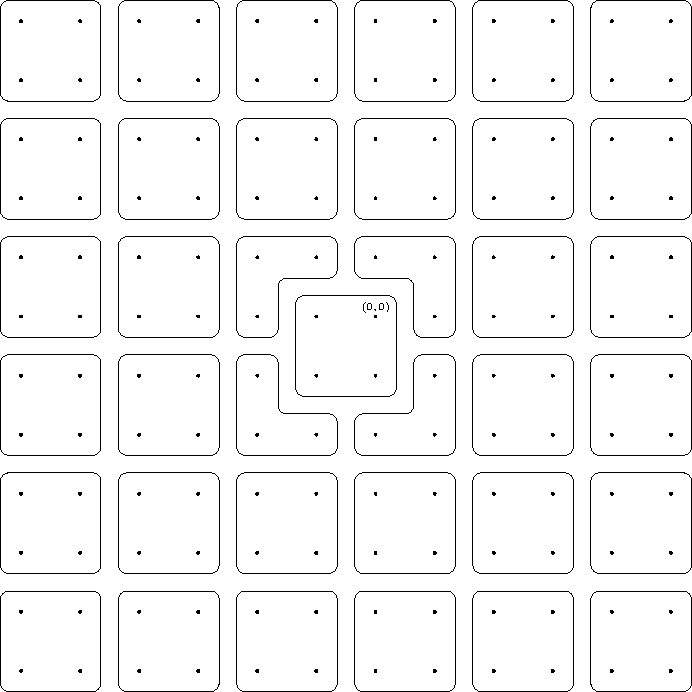
\includegraphics{figures/etendu-au-plan.pdf}\caption{Les points du plan regroupés par parent}
\end{figure}

\begin{lemma}\label{lemme-moins-de-peres}
Soit $E=\left\{p_0, p_1, p_2, p_3, p_4\right\}$ où $p_i \in \Z^2$ et $w \in \F^4$ tel que pour $i=0,1,2,3$ on a $p_{i+1} = p_{i} + w_i$, alors $\left|f(E)\right| \leq 4$.
\end{lemma}
\begin{proof}
L'arbre radix divise le plan en sections de $2\times2$ points partageant le même père. Par conséquent, au moins deux $p_i$ partagent le même père, d'où la borne $|f(E)| \leq 4$.
\end{proof}

\begin{theorem}\emph{\cite{BKP}.}
L'algorithme \parcours est linéaire.
\end{theorem}

\begin{proof}
On remarque d'abord que l'essentiel du temps passé dans \voisin est causé par l'appel récursif, puisque toutes les autres opérations sont d'ordre constant. Donc $\voisin$ est d'ordre $\O($h$)$ où $h$ est la hauteur de l'arbre. Cependant, un appel récursif n'est effectué sur un noeud que la première fois où l'un de ses enfants recherche son voisin, le résultat étant stocké directement au niveau de l'enfant la suite. Ainsi, pour tout noeud, \voisin est appelé un maximum de 16 fois (les quatre voisins de ses quatre enfants). Le temps total passé dans \voisin est donc proportionnel au nombre de noeuds créés. Reste à montrer que \parcours créé un nombre de noeuds proportionnel à $|w|$.

Soit $N$ tous les noeuds créés et $N_v \subseteq N$ les noeuds visités. On va montrer que le nombre total de noeuds créés est borné par un multiple du nombre de noeuds visités. Clairement, $|N_v| ≤ |N|$ et $|N_v| ≤ |w|$. De plus, on obtient $N$ à partir de $N_v$ grâce à $f$, $N = \bigcup_{i=0}^{h}f^i(N_v)$ donc
\begin{equation}\label{eq:nv-n}
|N| = \sum_{i=0}^{h} \left| f^i(N_v) \right|\text{.}
\end{equation}

Par construction chaque noeud ajouté à $N_v$ est voisin de son précédent. Le lemme \ref{lemme-moins-de-peres} s'applique et on regroupe les éléments par 5
\begin{equation}\label{eq:4-5emeNv}
|f(N_v)| ≤ 4 \left \lceil \frac{|N_v|}{5} \right \rceil ≤ \frac{4}{5}(|N_v| + 4)
\end{equation}

Le lemme \ref{lemme-parents-voisins} nous permet d'appliquer récursivement le lemme \ref{lemme-moins-de-peres} sur $f$. On combine donc les équations \ref{eq:nv-n} et \ref{eq:4-5emeNv} pour obtenir l'expression
\begin{equation}
|N| ≤ \sum_{i=0}^{h} \left| f^i(N_v) \right| ≤ \sum_{i=0}^{h} \left( \left( \frac{4}{5} \right)^i |N_v| + \sum_{j=0}^{i} \left( \frac{4}{5} \right)^j 4 \right) ≤ \cdots
\end{equation}
qu'on borne ensuite à l'aide de l'identité $\sum_{i=1}^\infty \left(\frac{4}{5}\right)^i=5$ pour finalement avoir
\begin{equation}
\cdots ≤ 5|N_v| + 4 \sum_{i=0}^{h} 5 ≤ 5|N_v| + 20h
\end{equation}

Puisque $h$ est précisément le nombre de bits requis pour écrire les coordonnées des points dans $N$, $h\in \O(\log n)$ et ainsi $|N| \in \O(n)$. Finalement, puisque $N_v ≤ |w|$ on a que $\parcours \in \O(|w|)$, tel que voulu.
\end{proof}

Le tableau \ref{fig:recapitulation-intersections} récapitule les avantages et les désavantages des trois méthodes de détection d'intersection présentées pour un chemin $w$ de longueur $|w|=n$

\begin{table}
\begin{tabular}{|l|l|l|l|}
\hline
Méthode & Complexité & Commentaires \\
\hline
Adressage direct & $\O(n^2)$ & \parbox{.6\textwidth}{\vspace{.33\baselineskip}
\begin{itemize}[leftmargin=*]
\item Rapide pour les petites valeurs de $n$.
\item Structure de données native en informatique.
\item On doit connaître $n$ au départ.
\end{itemize}\vspace{.25\baselineskip}}\\
\hline
Tri & $\O(n \log n)$ & \parbox{.6\textwidth}{\vspace{.33\baselineskip}
\begin{itemize}[leftmargin=*]
\item Méthode la moins gourmande en mémoire.
\item On n'a pas à connaître $n$ au départ.
\item Structures de données déjà implémentées sous forme de librairies.
\end{itemize}\vspace{.25\baselineskip}}\\
\hline
BKP & $\O(n)$ & \parbox{.6\textwidth}{\vspace{.33\baselineskip}
\begin{itemize}[leftmargin=*]
\item On n'a pas à connaître $n$ au départ.
\item Maintient sa performance même avec les chemins très longs.
\item Plus lent que les autres méthodes pour les chemins courts.
\end{itemize}\vspace{.25\baselineskip}}\\
\hline
\end{tabular}
\caption{Récapitulation des méthodes de détection d'intersection}\label{fig:recapitulation-intersections}
\end{table}

On en arrive à l'algorithme principal de ce chapitre.

\begin{algorithm}
	\fontsize{10}{10}\selectfont
	\begin{algorithmic}[1]
	\Require Un mot $w \in \F^*$ codant un chemin discret.
	\Ensure Un mot $w' \in F^*$ codant $\hull{w}$.
	\Function{hull}{$w$}
		\State Invoquer $\parcours$ sur le mot $w$ à partir de $(0,0)$. \label{initialisation}
		\State Soit $W$ un point de la factorisation standard. \label{c1a}
		\State Soit $V$ l'ensemble des voisins explicites de $W$. \label{c1b}
		\State $c \gets V_0$ \label{c1c}
		\State $w' = \text{Step}(c-W)$ \label{w'initialise} \label{c1d}
		\While {$c \neq W$ ou $|V| \neq 0$}\label{boucle}
			\State $turn \gets 2$
			\For{chaque voisin explicite $v$ de $c$}\label{pour-chaque-voisin}
				\State $\Delta \gets \text{Step}(v-c)$
				\If{$\left( \Delta - w'_{n-1} \right)+1 \mod 4 ≤ turn + 1 \mod 4$}
					\State $turn \gets \Delta - w'_{n-1}$
					\State $suivant \gets v$
				\EndIf
			\EndFor \label{pour-chaque-voisin-fin}
			\State $w' = w' \cdot \Delta$ \label{grow-w'}
			\State Retirer $c$ de $V$ \label{vider-grand-V}
			\State $c \gets suivant$
		\EndWhile
		\State \Return $w'$
	\EndFunction
	\end{algorithmic}
\caption{Algorithme \HULL}\label{algorithme-hull}
\end{algorithm}

On commence à la ligne \ref{initialisation} par construire l'arbre radix augmenté associé au mot $w$. En commençant au point $c=W$, on procède pour chaque position $c$
\begin{enumerate}
\item Extraire la lettre $\Delta\in\F$ associée au vecteur $\vec{cv}$ pour chaque voisin $v$ de $c$.
\item Déterminer le virage associé à chaque $\Delta$.
\item Choisir le virage le plus à droite, c'est à dire celui le plus proche de $3$.
\end{enumerate}
L'algorithme se termine lorsqu'on revient au point $W$.

\begin{theorem}[Justesse de l'algorithme \ref{algorithme-hull}.] Pour chaque mot $w\in\F^*$ l'algorithme \ref{algorithme-hull} calcule $\hull{w}$.
\end{theorem}

\begin{proof}
Soit $\hull{w}$ de longeur $k\in \N$. On utilise l'invariant de boucle suivant:

\blockquote{Au début de la $i$-ième itération de la boucle à la ligne \ref{boucle}, $w'$ est un préfixe de longeur $i$ du mot de contour associé à $\hull{w}$.}

L'invariant tient lors de la première itération de la boucle à la ligne \ref{boucle}, puisqu'à ce moment $w'$ a été initialisé à la ligne \ref{w'initialise}. On suppose donc que l'invariant tient encore au début de la $i$-ième itération. $w'$ est alors un préfixe de longeur $i$ de $\hull{w}$. Les lignes \ref{pour-chaque-voisin} à \ref{pour-chaque-voisin-fin} calculent la direction du voisin le plus à droite et la ligne \ref{grow-w'} concatène cette direction à $w'$. Par la règle de la main droite, choisir le voisin le plus à droite assure de demeurer sur l'enveloppe extérieure de $w$. Ainsi, à la fin de la $i$-ième itération, $w'$ est un préfixe du mot de contour associé à $\hull{w}$ de longueur $i+1$. Finalement, à la fin de la boucle, $w'$ est un préfixe de $\hull{w}$ de longueur $k$, autrement dit $w'=\hull{w}$. Notons que puisque tous les voisins de $W$ sont sur l'enveloppe externe, la ligne \ref{vider-grand-V} retire bien tous les éléments de $V$ ce qui garantit que l'algorithme se termine.
\end{proof}

Nous terminons maintenant cette section en démontrant que l'algorithme \ref{algorithme-hull} est linéaire en temps et en espace. On a déjà démontré que \parcours est linéaire en temps. On peut facilement obtenir $W$ lors du parcours initial sans aucun coût supplémentaire. Les lignes \ref{c1a}, \ref{c1b}, \ref{c1c} et \ref{c1d} s'exécutent toutes en temps constant. Ensuite, la boucle extérieure à la ligne \ref{boucle} est exécutée exactement $k$ fois, une fois pour chaque lettre de $w'$ et $|w'| ≤ |w|$. Pour chaque itération de la boucle extérieure, la boucle intérieure s'exécute un maximum de $4$ fois. Le temps total de la boucle est donc de $k(4 c_1 + c_2)$, où $c_1$ et $c_2$ sont des constantes appartenant à $\R$, ce qui montre bien que l'algorithme \ref{algorithme-hull} dans son ensemble est linéaire en temps. On termine la preuve en remarquant que l'arbre radix augmenté est linéaire en espace et qu'aucun nouveau noeud n'est créé après l'appel initial à \parcours.
% !TEX root = memoire.tex
\chapter{G\'en\'eration exaustive}\label{chapitre-generation}

\vspace{-1em}
Dans ce chapitre nous présentons un algorithme de génération exhaustive basé sur le parcours du bord extérieur d'un polyomino.

Si nous connaissons le polyomino à l'avance, il existe un parcours canonique de son bord de longueur minimale. Pour l'obtenir nous avons besoin de deux choses: un point de départ canonique sur le bord et une orientation du parcours. Ensuite, à partir de ce point de départ, on se déplace de manière à longer le bord du polyomino. 

Nous présentons la classe des polyominos ainsi énumérés ainsi que leur représentation à l'aide de pierres de \Go dans la section $1$. Dans la section $2$, nous décrirons un jeu basé sur le \Go dont une partie terminée représente un polyomino délimité par un nombre donné de pierres noires. Nous terminerons le chapitre avec la section $3$, où nous présentons l'algorithme de génération exhaustive ainsi qu'une spécialisation pour les polyominos avec différents types de trou.


\vspace{-1em}
\section{Les gominos}

%On considère les chemins codés par les lettres de l'alphabet $\mathcal{A}=\{0,1,2,3,4,5,6,7\}$. Un sous-ensemble $S\subseteq\Z^2$ est \emph{$4$-connexe} (resp. \emph{$8$-connexe}) si toute paire de points est reliée par un $4$-chemin (resp. $8$-chemin). Un \emph{polyomino} $P$ est un ensemble fini $4$-connexe, habituellement représenté à l'aide de carrés unités dans le plan $\Z^2$.

\vspace{-0.5em}
On considère $\Z^2$ comme une planche de \Go infinie et on y représente le contour extérieur $P^+$ d'un polyomino $P$ à l'aide de pierres noires, et le contour intérieur $P^-$ à l'aide de pierres blanches tel qu'illustré à la figure \ref{fig:polyomino-et-gomino}. 

\begin{definition}\label{def:gomino}
Un \emph{gomino} est une paire $G=\left( P^+,P^- \right)$ d'ensembles dans $\Z^2$ pour lesquels il existe un polyomino $P$ tel que $P^+$ est son contour extérieur et $P^-$ est son contour intérieur.
\end{definition}

\begin{figure}[h]
\centering
\begin{tikzpicture}[scale=.4, tile/.style={draw, blue!60!black, fill=blue!10, rectangle, inner sep=0.2cm}]
\draw[color=black!20] (-2.1,-1.1) grid (4.1,5.1);
\squarepath{(-1,2)}{66000222446602};
\node[draw=none,fill=none] at (5.5,2.5) {$\cong$}; 
\end{tikzpicture} 
\hspace{.5cm}
\begin{tikzpicture}[scale=.4, every node/.style={scale=.4, minimum size=1cm}, node distance=1cm] 
\goban{6}{6} 
\whitestonepath{(1,3)}{66000222446};
\blackstonepath{(0,3)}{667000122234455};
\end{tikzpicture}

\caption{Un polyomino simplement $4$-connexe et son gomino.}\label{fig:polyomino-et-gomino}
\end{figure}

L'analogie avec le \Go, autre que le fait d'utiliser des pierres noires et blanches, réside dans le fait que selon la terminologie du \Go, un polyomino simplement $4$-connexe $P$ avec son contour $P^+$ est le \emph{territoire noir}, et $P^+$ délimite ce territoire de façon minimale. L'algorithme décrit plus loin génère chaque gomino avec $n$ pierres noires, donc chaque polyomino de périmètre de site $n$, en plaçant tour à tour des pierres noires et blanches, comme le feraient deux joueurs de \Go.


\section{Un jeu bien solitaire}

Le jeu de \textit{Gomino} est d'une certaine façon une version simplifiée du jeu de \Go. D'une position initiale, deux joueurs $\B$ et $\W$ jouent sur une planche de jeu $\N \times \Z$ en laissant des pierres sur chaque point de la grille visité et libre jusque là. $\B$ a $n$ pierres noires en main et tente d'encercler un territoire en revenant à sa position d'origine, tandis que $\W$ essaie de l'en empêcher en plaçant des pierres blanches.

On décrit la séquence des positions successives de chacun des joueurs à l'aide deux fonctions
\[\B, \W: \N \to \N\times\Z,\]
dont on fixe les points de départ
\begin{equation}\label{CI}
\B(0)= (0,0)  \quad;\quad
\W(0) = (1,0).
\end{equation}

La notion suivante est utile pour décrire les $4$-trous.

\begin{definition}
Un \emph{motif en X} est un alignement de pierres $2\times2$ tel que l'une de ses diagonales est noire, et l'autre blanche.
\end{definition}

\begin{figure}[h!]
\centering

\begin{subfigure}[b]{.4\textwidth}
\centering
\begin{tikzpicture}[every node/.style={minimum size=1cm}, node distance=1cm]
\gobanc{2}{2}
\wm{(0,0)} \wm{(1,1)}
\bm{(0,1)} \bm{(1,0)}
\end{tikzpicture}
\end{subfigure}
\begin{subfigure}[b]{.4\textwidth}
\centering
\begin{tikzpicture}[every node/.style={minimum size=1cm}, node distance=1cm]
\gobanc{2}{2}
\bm{(0,0)} \bm{(1,1)}
\wm{(0,1)} \wm{(1,0)}
\end{tikzpicture}
\end{subfigure}
\caption{Motifs en X}
\end{figure}

\subsection{Position de départ et zones interdites}

Afin de rendre chaque parcours unique et éviter la répétition de polyominos par translation, on choisit une cellule du polyomino $P$, appellée la \emph{racine} de $P$. L'une des manières d'obtenir canoniquement une telle cellule est d'utiliser la factorisation standard tel qu'illustré  à la figure \ref{fig:NSEW} et de choisir la cellule ayant comme sommet le point $W$.

\begin{figure}
\centering
\shorthandoff{:}
\begin{tikzpicture}[polyomino/.style={black, fill=red, fill opacity=0.3, very thick}, >=latex, scale=0.5]
	\squarepath{(1,2)}{06200244202060};
	\draw[help lines, opacity=0.3] (-0.1,-0.1) grid (7.1, 7.1);
	\draw[very thick, opacity=0.3] (1,1) rectangle (6,6);
	\node[circle, draw, fill, inner sep=1, label=below left:{$W$}] at (1,2) {};
	\node[circle, draw, fill, inner sep=1, label=below right:{$S$}] at (3,1) {};
	\node[circle, draw, fill, inner sep=1, label=above right:{$E$}] at (6,5) {};
	\node[circle, draw, fill, inner sep=1, label=above left:{$N$}] at (3,6) {};
\end{tikzpicture}
\caption{Factorisation NSEW du contour}\label{fig:NSEW}
\end{figure}

Pour s'assurer de respecter les contraintes imposées par le choix de la racine, on interdit à $\B$ de jouer sous sa position initiale en colonne $0$ et à $\W$ de jouer sur la colonne $0$. Ces positions sont appelées \emph{zones interdites}.

\begin{figure}[H]
\centering
\begin{tikzpicture}
\goban{5}{5}
\node[opacity=0.25] at (0,0) {\blackstone};
\node at (0,0) [forbidden sign,line width=0.3ex,draw=red]{};
\node[opacity=0.25] at (0,1) {\blackstone};
\node at (0,1) [forbidden sign,line width=0.3ex,draw=red]{};
\node at (0,2) {\blackstone};
\node at (1,2) {\whitestone};
\node[opacity=0.25] at (0,3) {\whitestone};
\node at (0,3) [forbidden sign,line width=0.3ex,draw=red]{};
\node[opacity=0.25] at (0,4) {\whitestone};
\node at (0,4) [forbidden sign,line width=0.3ex,draw=red]{};
\end{tikzpicture}

\caption{Position de départ et zones interdites}
\end{figure}

\subsection{Règles de déplacement}
Le joueur $\B$ commence, et les joueurs jouent à tour de de rôle (figure \ref{figure:anatomie-coup}).

La liste des coups possibles est illustrée à la figure \ref{fig:regles-de-deplacement}. La pierre noire marquée en vert indique la position de $\B$, tandis que la pierre blanche marquée en vert qui y est $4$-connexe indique celle de $\W$. Les règles sont les suivantes:

\begin{figure}
\centering
\begin{subfigure}[b]{.3\textwidth}
\centering
\begin{tikzpicture}
\gobanc{3}{3}
\wm{(1,0)}
\bm{(1,1)}
\end{tikzpicture}
\caption{Position initiale}
\end{subfigure}
\begin{subfigure}[b]{.3\textwidth}
\centering
\begin{tikzpicture}
\gobanc{3}{3}
\wm{(1,0)}
\bm{(1,1)}
\bm{(2,2)}
\markstone{2}{2}
\end{tikzpicture}
\caption{Coup de $\B$}
\end{subfigure}
\begin{subfigure}[b]{.3\textwidth}
\centering
\begin{tikzpicture}
\gobanc{3}{3}
\whitestonepath{(1,0)}{4220}
\bm{(1,1)}
\bm{(2,2)}
\markstone[green!90!black]{0}{0}
\markstone[green!90!black]{0}{1}
\markstone[green!90!black]{0}{2}
\markstone[green!90!black]{1}{2}
\end{tikzpicture}
\caption{Réplique de $\W$}
\end{subfigure}
\caption{L'anatomie d'un coup}\label{figure:anatomie-coup}
\end{figure}




\begin{figure}[h!]
\begin{center}
\tikzstyle{level 1}=[sibling angle=(360/8), level distance=22mm]
\tikzstyle{level 2}=[sibling angle=(360/8), level distance=28mm]
\tikzstyle{every node}=[]
\tikzstyle{edge from parent}=[->, draw]
\begin{tikzpicture}[auto, >=latex, grow cyclic, clockwise from=90]
\node (ref) {\kifuc[scale=.2]{3}{\wm{(1,0)}\bm{(1,1)}}}
child {node[scale=.3] (a)  {\begin{tikzpicture}[every node/.style={minimum size=1cm}, node distance=1cm]
	\gobanc{3}{3};
	\wm{(1,0)}
	\bm{(1,1)}
	\bm{(1,2)}
	\markstone{1}{2};
\end{tikzpicture}}
  child[clockwise from=(90)] {node[scale=.7]{\begin{tikzpicture}[every node/.style={minimum size=1cm}, node distance=1cm]
	\goban{3}{3}
	\wm{(1,0)}
	\bm{(1,1)}
	\bm{(1,2)}
	\wm{(0,0)}
	\wm{(0,1)}
	\wm{(0,2)}	
	\markstone{0}{0}
	\markstone{0}{1}
	\markstone{0}{2}
\end{tikzpicture}
} edge from parent}
edge from parent}
child {node[scale=.3] (b) {\begin{tikzpicture}[every node/.style={minimum size=1cm}, node distance=1cm]
	\gobanc{3}{3};
	\wm{(1,0)}
	\bm{(1,1)}
	\bm{(2,2)}
	\markstone{2}{2};
\end{tikzpicture}}
  child[clockwise from=(45)] {node[scale=.7]{\begin{tikzpicture}[every node/.style={minimum size=1cm}, node distance=1cm]
	\goban{3}{3}
	\wm{(1,0)}
	\bm{(1,1)}
	\bm{(2,2)}
	\wm{(0,0)}
	\wm{(0,1)}
	\wm{(0,2)}	
	\wm{(1,2)}
	\markstone{0}{0}
	\markstone{0}{1}
	\markstone{0}{2}
	\markstone{1}{2}
\end{tikzpicture}
} edge from parent}
edge from parent[swap]}
child {node[scale=.3] (c) {\begin{tikzpicture}[every node/.style={minimum size=1cm}, node distance=1cm]
	\gobanc{3}{3};
	\wm{(1,0)}
	\bm{(1,1)}
	\bm{(2,1)}
	\markstone{2}{1};
\end{tikzpicture}}
  [clockwise from=0]
  child {node[scale=.7]{\begin{tikzpicture}[every node/.style={minimum size=1cm}, node distance=1cm]
	\goban{3}{3}
	\wm{(1,0)}
	\bm{(1,1)}
	\bm{(2,1)}
	\wm{(0,0)}
	\wm{(0,1)}
	\wm{(0,2)}	
	\wm{(1,2)}
	\wm{(2,2)}
	\markstone{0}{0}
	\markstone{0}{1}
	\markstone{0}{2}
	\markstone{1}{2}
	\markstone{2}{2}
\end{tikzpicture}
} edge from parent}
edge from parent[swap]}
child {node[scale=.3] (d) {n\begin{tikzpicture}[every node/.style={minimum size=1cm}, node distance=1cm]
	\gobanc{3}{3};
	\wm{(1,0)}
	\bm{(1,1)}
	\bm{(2,0)}
	\markstone{2}{0};
\end{tikzpicture}}
  [clockwise from=-45]
  child[sibling angle=45] {node[scale=.7]{\begin{tikzpicture}[every node/.style={minimum size=1cm}, node distance=1cm]
	\goban{3}{3}
	\wm{(1,0)}
	\bm{(1,1)}
	\bm{(2,0)}
	\wm{(0,0)}
	\wm{(0,1)}
	\wm{(0,2)}	
	\wm{(1,2)}
	\wm{(2,2)}
	\wm{(2,1)}
	\markstone{0}{0}
	\markstone{0}{1}
	\markstone{0}{2}
	\markstone{1}{2}
	\markstone{2}{2}
	\markstone{2}{1}
\end{tikzpicture}
} edge from parent}
 edge from parent[swap]}
child[missing] {}
child {node[scale=.3] (B) {\begin{tikzpicture}[every node/.style={minimum size=1cm}, node distance=1cm]
	\gobanc{3}{3};
	\wm{(1,0)}
	\bm{(1,1)}
	\bm{(0,0)}
	\markstone{0}{0};
\end{tikzpicture}}
  [clockwise from=-180+45]
  child {node[scale=.7]{\begin{tikzpicture}[every node/.style={minimum size=1cm}, node distance=1cm]
	\gobanc{3}{3};
	\wm{(1,0)}
	\bm{(1,1)}
	\bm{(0,0)}
\end{tikzpicture}} edge from parent}
 edge from parent}
child {node[scale=.3] (C) {\begin{tikzpicture}[every node/.style={minimum size=1cm}, node distance=1cm]
	\gobanc{3}{3};
	\wm{(1,0)}
	\bm{(1,1)}
	\bm{(0,1)}
	\markstone{0}{1};
\end{tikzpicture}}
  [clockwise from=(180)]
  child {node[scale=.7]{\begin{tikzpicture}[every node/.style={minimum size=1cm}, node distance=1cm]
	\gobanc{3}{3};
	\wm{(1,0)}
	\bm{(1,1)}
	\bm{(0,1)}
	\wm{(0,0)}
	\markstone{0}{0};
\end{tikzpicture}} edge from parent}
edge from parent}
child {node[scale=.3] (D) {\begin{tikzpicture}[every node/.style={minimum size=1cm}, node distance=1cm]
	\gobanc{3}{3};
	\wm{(1,0)}
	\bm{(1,1)}
	\bm{(0,2)}
	\markstone{0}{2};
\end{tikzpicture}}
  [clockwise from=(180-45)]
  child[sibling angle=45] {node[scale=.7]{\begin{tikzpicture}[every node/.style={minimum size=1cm}, node distance=1cm]
	\gobanc{3}{3};
	\wm{(1,0)}
	\bm{(1,1)}
	\bm{(0,2)}
	\wm{(0,0)}
	\wm{(0,1)}
	\markstone{0}{0};
	\markstone{0}{1};
\end{tikzpicture}} edge from parent}
edge from parent}
;
\end{tikzpicture}
\end{center}
\caption{Coups permis (à rotation près)}
\label{fig:regles-de-deplacement}
\end{figure}

\begin{itemize}
\item[$\B$:] ce joueur se déplace exactement d'un pas dans son $8$-voisinage excluant la zone interdite et les positions déjà occupées par des pierres blanches. On remarque que seuls les déplacements vers des intersections libres augmentent le nombre de pierres noires en jeu. De plus, $\B$ doit jouer son premier coup en direction \ocr{7}. Cette contrainte force $\B$ à parcourir le bord du polyomino en sens anti-horaire.

\item[$\W$:] ce joueur doit terminer son coup dans le $4$-voisinage de $\B$ en un nombre minimal de pas, de $0$ à $6$ selon le coup de $\B$. Il peut le faire en effectuant autant de pas qu'il le faut sur les intersections vides ou sur les pierres blanches dans le $8$-voisinage de la position précédente de $\B$ tout en respectant les conditions suivantes:

\begin{enumerate}
\item \emph{Règle de la main droite.} À la fin de chaque tour, $\W$ doit être situé à gauche de la flèche décrivant le dernier coup de $\B$.

Cette règle force $\W$ à rester à l'intérieur du polyomino dont le bord extérieur est construit par $\B$.

\item \emph{Règle des trous.} $\W$ ne peut en aucun cas former de motif en X.

La règle des trous évite de créer des polyominos contenant des $8$-trous et ainsi assure que tous les polyominos générés par l'algorithme seront simplement $4$-connexe. Cette contrainte sera relâchée plus tard lorsque nous adapterons l'algorithme pour obtenir les polyominos contenant les différents types de trous.
\end{enumerate}
\end{itemize}

\vspace{-0.5em}
Pour comprendre l'ajout de plusieurs pierres blanches en un seul coup, on doit se rappeler que par définition, $\B$ encercle $\W$ avec un minimum de pierres. Chaque coup de $\B$ nous révèle donc un peu plus d'information sur $\W$. En particulier, si $\W$ peut jouer une pierre alors on sait que cet emplacement fait bien partie de $\W$ puisque dans le cas contraire $\B$ aurait tout simplement joué là au tour précédent et ainsi bloqué $\W$.

On remarque aussi que la séquence qui mène à l'ajout de 6 pierres est interdite par la règle des trous et donc n'est pas un coup valide pour $\W$. Elle sera par contre utilisée plus loin pour générer les polyominos simplement $8$-connexes.

Finalement, la restriction de $\W$ sur la colonne $0$ garanti que si $\B$ joue sur la colonne $-1$ on a une victoire de $\W$. Puisqu'on cherche à énumérer les victoires de $\B$, on évitera d'y jouer.

\vspace{-0.5em}
\subsection{Fin de partie}

\vspace{-0.5em}
On dit que \emph{$\B$ gagne} s'il parvient à revenir à sa position d'origine. Dans ce cas, les chemins parcourus par $\B$ et $\W$ décrivent respectivement le contour extérieur et intérieur d'un unique polyomino $P$.

Si à n'importe quelle étape, $\W$ est incapable de rejoindre le $4$-voisinage de $\B$ en utilisant un coup permis, alors $\W$ gagne. De plus, quand aucune séquence de coups ne mène à une victoire de $\B$, alors $\W$ gagne. En conséquence, il y a bijection entre les polyominos et les parties de Gomino gagnées par $\B$.

\begin{theorem}\label{thm:G=P}
Tout polyomino simplement $4$-connexe $P$ est décrit par une unique partie de gomino $G$ gagnée par $\B$.
\end{theorem}

\begin{proof}
Soit $P$ un polyomino simplement $4$-connexe, $P^+$ et $P^-$ ses contours extérieurs et intérieurs. On construit, par induction, une partie de Gomino qui décrit $P$ et on montre que cette partie est unique.

On débute avec $\B(0)$ et $\W(0)$ tel que décrit par l'équation \eqref{CI}, et on identifie $\W(0)$ à la racine de $P$. Puisque le premier coup de $\B$ doit absolument être $0$, on a que $\B(1)=(1,-1)$, qui est un point de $P^+$, et $\W(1)=(1,0)$, qui est un point de $P^-$.

Supposons maintenant que $\B$ a déjà joué $n$ coups tels que chaque pierre noire placée jusqu'à maintenant est dans $P^+$ et chaque pierre blanche est dans $P^-$. Soit $\vec{b}_n$ la flèche de $\B(n-1)$ vers $\B(n)$. À l'étape $n$, nous sommes, à rotation près, dans la situation illustrée à la figure \ref{fig:ordre}. Certaines intersections peuvent contenir des pierres. On numérote les intersections en commençant à $0$ à partir de $\W(n)$.

\begin{figure}[h!]
\centering
\begin{tikzpicture}[every node/.style={scale=1}, marker/.style={fill=brown, inner sep=0, circle}]
	\gobanc{3}{3}
	\wm{(1,0)}
	\bm{(1,1)}
	\markstone[green!90!black]{1}{0}
	\markstone{1}{1}
\node[marker] at (0,0) {\circled{0}};
\node[marker] at (0,1) {\circled{1}};
\node[marker] at (0,2) {\circled{2}};
\node[marker] at (1,2) {\circled{3}};
\node[marker] at (2,2) {\circled{4}};
\node[marker] at (2,1) {\circled{5}};
\node[marker] at (2,0) {\circled{6}};
\end{tikzpicture}
\caption{Ordre du $8$-voisinage}
\label{fig:ordre}
\end{figure}

On remarque qu'en numérotant le voisinage de $\B(n)$ en sens horaire en commençant à $\W(n)$, le point $\B(n+1)$ est le premier point de $P^+$ rencontré. En effet, lorsque $\B$ place une pierre en $i$, $\W$ réplique en plaçant ses pierres en $1,2,\dots, i-1$, ce qu'il peut toujours faire puisque ces positions sont libres et dans le $8$-voisinage de $\B(n)$. S'il existait une position $j<i$ contenant déjà une pierre noire, alors $\W$ serait incapable de se connecter à la nouvelle position de $\B$ et serait victorieux donc la partie ne représenterait pas $P$. De même, s'il existe une position $j<i$ qui contiendra éventuellement une pierre noire, $\B$ doit obligatoirement jouer sur ce point de $P^+$, sinon $\W$ y placera une pierre blanche et notre gomino ne représentera plus $P$.
\end{proof}

\paragraph*{Remarque:} Une conséquence directe du théorème 1 est que la séquence des coups joués par $\B$ lors d'une victoire, codée par un mot sur $\mathcal{A}$, est suffisante pour décrire un polyomino unique. Par exemple, le polyomino illustré à la figure \ref{fig:polyomino-et-gomino} est encodé par le mot $w=\ocr{700012223445566}$.



\section{L'algorithme de génération}

\vspace{-0.5em}
Nous utilisons maintenant la bijection entre les parties de Gomino et les polyominos pour décrire notre principal algorithme qui permet la génération exhaustive des polyominos simplement $4$-connexes. Nous parlerons simplement de \emph{l'algorithme des gominos}. Lorsque nous faisons référence à une partie de gomino, celle-ci peut être inachevée.

\vspace{-0.5em}
\paragraph{\bf L'algorithme des gominos.} {\it L'algorithme accepte en entrée une partie de gomino de $n$ coups et retourne en sortie la liste des parties de $(n+1)$ coups possibles à partir de ce point.

\vspace{-0.5em}
\begin{enumerate}
\item \emph {Construire la liste des coups valides}

D'abord le coup de $\B$: toute intersection vide ou contenant une pierre noire dans le $8$-voisinage de la position actuelle de $\B$ est un coup valide. $\W$ répond immédiatement et comme il est montré à la figure \ref{fig:regles-de-deplacement}, a un seul coup possible. Si $\W$ est incapable de jouer, rejeter ce coup immédiatement. Sinon, l'ajouter à la liste.

\item \emph{Créer de nouvelles parties}

Pour chaque coup valide, créer une copie de la partie actuelle, y jouer ce coup et ajouter la partie à l'ensemble des nouvelles parties. Pour chaque partie de $n$ coups, l'algorithme peut créer jusqu'à sept nouvelles parties de $(n+1)$ coups. La partie reçue en paramètre par l'algorithme n'est plus utilisée par la suite et peut être effacée à ce moment.

\item \emph{Comptabiliser les victoires}

Les conditions de victoires sont vérifiées sur chaque nouvelle partie. Les victoires de $\W$ sont rejetées et les victoires de $\B$ sont conservées (ce sont nos polyominos). Puis les autres parties sont ajoutées à l'ensemble des parties en cours.

\item \emph{Appliquer récursivement}

On applique ensuite l'algorithme récursivement sur chacune des parties en cours, jusqu'à ce que cet ensemble soit vide. Puisque chaque partie est indépendante des autres, cette étape peut être traitée en parallèle.
\end{enumerate}

}


\vspace{-0.5em}
\subsection{$4$-trous} \label{subsection:4-trous}

\vspace{-0.5em}
Nous présentons maintenant une extension de l'algorithme de base qui permet de générer les polyominos simplement $8$-connexes en retirant la règle des trous. Le coup blanc \ocr{422006} devient alors valide et décrit un trou d'aire $1$.

Notons que la preuve du théorème \ref{thm:G=P} ne fait aucune mention de $4$-trous. Conséquemment, le théorème reste vrai pour les polyominos simplement $8$-connexes incluant des motifs en X. Bien que ces motifs soient permis pour les polyominos simplement $8$-connexes, nous pouvons les utiliser pour compter les $4$-trous.

\begin{proposition}
Si un gomino $G$ décrit un polyomino simplement $8$-connexe $P$, alors il y a autant de motif en X dans $G$ qu'il y a de $4$-trous dans $P$.
\end{proposition}

\vspace{-0.5em}
\begin{proof}
Procédons par induction sur le nombre de $4$-trous dans un polyomino $P$.
Considérons tout d'abord le cas d'un seul $4$-trou. Il y a au moins un motif en X, puisque c'est le seul motif qui bloque tout $4$-chemin de l'intérieur vers l'extérieur du trou tout en permettant l'existence de $8$-chemin. S'il y avait un $4$-chemin de l'intérieur vers l'extérieur, alors ce ne serait pas un trou. D'un autre coté, si on suppose l'existence de deux motifs en X, alors il existe deux $8$-chemins reliant l'intérieur du trou à l'extérieur. Prenons deux points, par exemple $z$ à l'intérieur du trou, et $w$ à l'extérieur. On peut relier $z$ et $w$ par deux chemins différents qui ne croisent pas $P$, chacun passant par l'un des motifs en X. Ces deux chemins forment un $8$-chemin fermé contenant une partie de $P$ (la \emph{partie intérieure}). Une autre partie de $P$ est à l'extérieur du chemin fermé (la \emph{partie extérieure}), sinon $z$ ne serait pas à l'intérieur d'un $4$-trou. Finalement, il n'existe pas de $4$-chemin qui relie la partie intérieure à la partie extérieure sans croiser le $8$-chemin donc $P$ n'est pas $4$-connexe: une contradiction. Il n'y a donc qu'un seul motif en X.

Supposons maintenant que pour tout polyomino simplement $8$-connexe avec $(n-1)$ $4$-trous, il y a exactement $(n-1)$ motif en X. Soit $P$ un polyomino simplement $8$-connexe avec $n$ $4$-trous. Il y a au moins un $4$-trou qui peut être rempli afin d'obtenir le polyomino simplement $8$-connexe $P'$. Nous appellerons ce $4$-trou le $n^{\text{ième}}$ trou. Le polyomino $P'$ a exactement $(n-1)$ $4$-trou, alors par hypothèse d'induction il possède aussi $(n-1)$ motifs en X. Par le même raisonnement que pour le cas initial, l'ajout du $n^{\text{ième}}$ trou ajoute exactement un motif en X. $P$ a donc $n$ motifs en X, tel que voulu.
\end{proof}



\subsection{$8$-trous}\label{subsection:8-trous}

Pour obtenir les $8$-trous, nous allons utiliser une version légèrement modifiée de l'algorithme de base sur les positions libres à l'intérieur d'un gomino. Ces positions devront être remplies par des pierres noires ou blanches jusqu'à ce que $\W$ n'ait plus de \emph{libertés} pour réutiliser la terminologie du \Go, c'est à dire qu'il ne reste plus aucune intersection libre dans le $4$-voisinage des pierres blanches. On remarquera qu'il n'y a jamais d'intersections libres dans les $4$-trous $8$-connectés à l'extérieur: ces trous sont déjà générés correctement par l'algorithme étendu présenté à la section \ref{subsection:4-trous}.

\begin{figure}[h]
\centering
\begin{tikzpicture}[scale=.4, every node/.style={scale=.4, minimum size=1cm}, node distance=1cm]
\goban{7}{7}
\bm{(1,6)}\bm{(2,6)}\bm{(3,6)}\bm{(4,6)}\bm{(5,6)}\bm{(0,5)}\wm{(1,5)}\wm{(2,5)}\wm{(3,5)}\wm{(4,5)}\wm{(5,5)}\bm{(6,5)}\bm{(0,4)}\wm{(1,4)}\wm{(5,4)}\bm{(6,4)}\bm{(0,3)}\wm{(1,3)}\wm{(5,3)}\bm{(6,3)}\bm{(0,2)}\wm{(1,2)}\wm{(5,2)}\bm{(6,2)}\bm{(0,1)}\wm{(1,1)}\wm{(2,1)}\wm{(3,1)}\wm{(4,1)}\wm{(5,1)}\bm{(6,1)}\bm{(1,0)}\bm{(2,0)}\bm{(3,0)}\bm{(4,0)}\bm{(5,0)}
\bm{(2,2)}
\bm{(2,3)}
\bm{(2,4)}
\bm{(3,4)}
\bm{(4,4)}
\bm{(4,3)}
\bm{(4,2)}
\bm{(3,2)}
\end{tikzpicture}
\caption{Un gomino sans libertés pour $\W$}
\end{figure}


Comme pour l'algorithme des gominos, les trous sont énumérés en fixant leur cellule en bas à gauche. Pour ce faire, on exécute l'algorithme avec chaque position de départ possible, de bas en haut et de gauche à droite. Une position de départ valide pour le $\B$ est à droite d'une pierre blanche. Cette pierre blanche est la position initiale de $\W$. $\B$ gagne si les deux joueurs reviennent à leurs positions initiales. Ceci garantit que le chemin suivi par $\W$ est fermé, et ainsi délimite bien un $8$-trou. Cette fois cependant, $\W$ peut dépasser son point de départ en réponse à $\B$. Ainsi, $\B$ gagne dès que $\W$ revient à son point de départ, même si $\W$ n'as pas terminé son coup. 

\begin{figure}[h]
\centering
\begin{subfigure}[b]{.18\textwidth}{
\centering
\begin{tikzpicture}[scale=.3, every node/.style={scale=.3, minimum size=1cm}, node distance=1cm]
\goban{6}{6}
\bm{(1,5)}\bm{(2,5)}\bm{(3,5)}\bm{(4,5)}\bm{(0,4)}\wm{(1,4)}\wm{(2,4)}\wm{(3,4)}\wm{(4,4)}\bm{(5,4)}\bm{(0,3)}\wm{(1,3)}\wm{(4,3)}\bm{(5,3)}\bm{(0,2)}\wm{(1,2)}\wm{(4,2)}\bm{(5,2)}\bm{(0,1)}\wm{(1,1)}\wm{(2,1)}\wm{(3,1)}\wm{(4,1)}\bm{(5,1)}\bm{(1,0)}\bm{(2,0)}\bm{(3,0)}\bm{(4,0)}
\end{tikzpicture}
\caption{A gomino}\label{letrou}
}\end{subfigure}
\begin{subfigure}[b]{.18\textwidth}{
\centering
\begin{tikzpicture}[scale=.3, every node/.style={scale=.3, minimum size=1cm}, node distance=1cm]
\goban{6}{6}
\bm{(1,5)}\bm{(2,5)}\bm{(3,5)}\bm{(4,5)}\bm{(0,4)}\wm{(1,4)}\wm{(2,4)}\wm{(3,4)}\wm{(4,4)}\bm{(5,4)}\bm{(0,3)}\wm{(1,3)}\wm{(4,3)}\bm{(5,3)}\bm{(0,2)}\wm[\Large{$\bigstar$}]{(1,2)}\wm{(4,2)}\bm{(5,2)}\bm{(0,1)}\wm{(1,1)}\wm{(2,1)}\wm{(3,1)}\wm{(4,1)}\bm{(5,1)}\bm{(1,0)}\bm{(2,0)}\bm{(3,0)}\bm{(4,0)}
\bm[\Large{$\bigstar$}]{(2,2)}
\end{tikzpicture}
\caption{Position 1}
}\end{subfigure}
\begin{subfigure}[b]{.18\textwidth}{
\centering
\begin{tikzpicture}[scale=.3, every node/.style={scale=.3, minimum size=1cm}, node distance=1cm]
\goban{6}{6}
\bm{(1,5)}\bm{(2,5)}\bm{(3,5)}\bm{(4,5)}\bm{(0,4)}\wm{(1,4)}\wm{(2,4)}\wm{(3,4)}\wm{(4,4)}\bm{(5,4)}\bm{(0,3)}\wm[\Large{$\bigstar$}]{(1,3)}\wm{(4,3)}\bm{(5,3)}\bm{(0,2)}\wm{(1,2)}\wm{(4,2)}\bm{(5,2)}\bm{(0,1)}\wm{(1,1)}\wm{(2,1)}\wm{(3,1)}\wm{(4,1)}\bm{(5,1)}\bm{(1,0)}\bm{(2,0)}\bm{(3,0)}\bm{(4,0)}
\wm{(2,2)}
\bm[\Large{$\bigstar$}]{(2,3)}
\end{tikzpicture}
\caption{Position 2}
}\end{subfigure}
\begin{subfigure}[b]{.18\textwidth}{
\centering
\begin{tikzpicture}[scale=.3, every node/.style={scale=.3, minimum size=1cm}, node distance=1cm]
\goban{6}{6}
\bm{(1,5)}\bm{(2,5)}\bm{(3,5)}\bm{(4,5)}\bm{(0,4)}\wm{(1,4)}\wm{(2,4)}\wm{(3,4)}\wm{(4,4)}\bm{(5,4)}\bm{(0,3)}\wm{(1,3)}\wm{(4,3)}\bm{(5,3)}\bm{(0,2)}\wm{(1,2)}\wm{(4,2)}\bm{(5,2)}\bm{(0,1)}\wm{(1,1)}\wm{(2,1)}\wm{(3,1)}\wm{(4,1)}\bm{(5,1)}\bm{(1,0)}\bm{(2,0)}\bm{(3,0)}\bm{(4,0)}
\wm[\Large{$\bigstar$}]{(2,2)}
\wm{(2,3)}
\bm[$\bigstar$]{(3,2)}
\end{tikzpicture}
\caption{Position 3}
}\end{subfigure}
\begin{subfigure}[b]{.18\textwidth}{
\centering
\begin{tikzpicture}[scale=.3, every node/.style={scale=.3, minimum size=1cm}, node distance=1cm]
\goban{6}{6}
\bm{(1,5)}\bm{(2,5)}\bm{(3,5)}\bm{(4,5)}\bm{(0,4)}\wm{(1,4)}\wm{(2,4)}\wm{(3,4)}\wm{(4,4)}\bm{(5,4)}\bm{(0,3)}\wm{(1,3)}\wm{(4,3)}\bm{(5,3)}\bm{(0,2)}\wm{(1,2)}\wm{(4,2)}\bm{(5,2)}\bm{(0,1)}\wm{(1,1)}\wm{(2,1)}\wm{(3,1)}\wm{(4,1)}\bm{(5,1)}\bm{(1,0)}\bm{(2,0)}\bm{(3,0)}\bm{(4,0)}
\wm{(2,2)}
\wm[\Large{$\bigstar$}]{(2,3)}
\wm{(3,2)}
\bm[\Large{$\bigstar$}]{(3,3)}
\end{tikzpicture}
\caption{Position 4}\label{fig:hole.minimal}
}\end{subfigure}
\caption{Les quatres positions initiales pour énumérer les trous de \ref{letrou}}
\label{fig:positions-initiales-trous}
\end{figure}

En plus des nouvelles positions de départ et conditions de fin, nous devons ajouter un nouveau coup pour $\B$ afin de pouvoir générer tous les trous. Ainsi, à son premier coup, $\B$ peut maintenant gagner immédiatement en restant sur place. $\W$ est alors forcé de faire un tour complet autour de $\B$, terminant la partie. Ce coup est nécessaire et suffisant pour produire les trous d'une seule pierre qui seraient autrement oubliés.

Finalement, lors d'une victoire de $\B$ où $\W$ est à court de libertés on a un polyomino avec ses trous complètement spécifié, sinon on applique récursivement l'algorithme sur les intersections encore libres. Après avoir énuméré tous les trous avec un certain $\B(0)$ et $\W(0)$, on place une pierre blanche sur $\B(0)$ et relance l'algorithme avec la position de départ suivante. La figure \ref{fig:positions-initiales-trous} illustre les différentes positions de départ utilisées pour générer les trous d'un polyomino.


\subsection{Optimisations}
Afin d'éliminer le plus rapidement possible un nombre maximal de parties où $\B$ perd, on conservera pour chaque intersection le nombre de pierres noires minimales requises pour revenir à l'origine. Le joueur noir pourra éviter de jouer sur des intersections inutilement "loin". À la figure \ref{fig:nombre-minimal-pierres} et à moins de mention contraire dans le reste de ce document, seules les intersections atteignables selon l'algorithme sont affichées.

\begin{figure}
\centering
\begin{subfigure}[b]{.4\textwidth}
\scalebox{.7}{
\begin{tikzpicture}[dist/.style={fill=brown, inner sep=0, circle}]\goban{7}{7};\bm{(1, 2)}\bm{(0, 3)}\wm{(1, 3)}
\node[dist] at (0,0) {\circled{$4$}};
\node[dist] at (1,0) {\circled{$4$}};
\node[dist] at (2,0) {\circled{$4$}};
\node[dist] at (3,0) {\circled{$4$}};
\node[dist] at (4,0) {\circled{$5$}};
\node[dist] at (5,0) {\circled{$5$}};
\node[dist] at (6,0) {\circled{$6$}};
\node[dist] at (0,1) {\circled{$3$}};
\node[dist] at (1,1) {\circled{$3$}};
\node[dist] at (2,1) {\circled{$3$}};
\node[dist] at (3,1) {\circled{$4$}};
\node[dist] at (4,1) {\circled{$4$}};
\node[dist] at (5,1) {\circled{$5$}};
\node[dist] at (6,1) {\circled{$6$}};
\node[dist] at (0,2) {\circled{$3$}};
\node[dist, fill=none, white] at (1,2) {\circled{$2$}};
\node[dist] at (2,2) {\circled{$3$}};
\node[dist] at (3,2) {\circled{$3$}};
\node[dist] at (4,2) {\circled{$4$}};
\node[dist] at (5,2) {\circled{$5$}};
\node[dist] at (6,2) {\circled{$6$}};
\node[dist] at (2,3) {\circled{$2$}};
\node[dist] at (3,3) {\circled{$3$}};
\node[dist] at (4,3) {\circled{$4$}};
\node[dist] at (5,3) {\circled{$5$}};
\node[dist] at (6,3) {\circled{$6$}};
\node[dist] at (0,4) {\circled{$1$}};
\node[dist] at (1,4) {\circled{$1$}};
\node[dist] at (2,4) {\circled{$2$}};
\node[dist] at (3,4) {\circled{$3$}};
\node[dist] at (4,4) {\circled{$4$}};
\node[dist] at (5,4) {\circled{$5$}};
\node[dist] at (6,4) {\circled{$6$}};
\node[dist] at (0,5) {\circled{$2$}};
\node[dist] at (1,5) {\circled{$2$}};
\node[dist] at (2,5) {\circled{$2$}};
\node[dist] at (3,5) {\circled{$3$}};
\node[dist] at (4,5) {\circled{$4$}};
\node[dist] at (5,5) {\circled{$5$}};
\node[dist] at (6,5) {\circled{$6$}};
\node[dist] at (0,6) {\circled{$3$}};
\node[dist] at (1,6) {\circled{$3$}};
\node[dist] at (2,6) {\circled{$3$}};
\node[dist] at (3,6) {\circled{$3$}};
\node[dist] at (4,6) {\circled{$4$}};
\node[dist] at (5,6) {\circled{$5$}};
\node[dist] at (6,6) {\circled{$6$}};
\begin{scope}\pgfsetfading{fading3}{\pgftransformshift{\pgfpoint{1cm}{2cm}}};\fill [green, even odd rule] (1, 2) circle (.6) circle (.45);\end{scope}
\end{tikzpicture}
} \end{subfigure}
\begin{subfigure}[b]{.4\textwidth}
\scalebox{.7}{
\begin{tikzpicture}[dist/.style={fill=brown, inner sep=0, circle}]\goban{7}{7};\bm{(1, 2)}\bm{(0, 3)}\wm{(1, 3)}\bm{(2, 2)}
\node[dist] at (0,0) {\circled{$4$}};
\node[dist] at (1,0) {\circled{$4$}};
\node[dist] at (2,0) {\circled{$4$}};
\node[dist] at (3,0) {\circled{$4$}};
\node[dist] at (4,0) {\circled{$4$}};
\node[dist] at (5,0) {\circled{$5$}};
\node[dist] at (0,1) {\circled{$3$}};
\node[dist] at (1,1) {\circled{$3$}};
\node[dist] at (2,1) {\circled{$3$}};
\node[dist] at (3,1) {\circled{$3$}};
\node[dist] at (4,1) {\circled{$4$}};
\node[dist] at (5,1) {\circled{$5$}};
\node[dist] at (0,2) {\circled{$3$}};
\node[dist, fill=none, white] at (1,2) {\circled{$2$}};
\node[dist, fill=none, white] at (2,2) {\circled{$2$}};
\node[dist] at (3,2) {\circled{$3$}};
\node[dist] at (4,2) {\circled{$4$}};
\node[dist] at (5,2) {\circled{$5$}};
\node[dist] at (2,3) {\circled{$2$}};
\node[dist] at (3,3) {\circled{$3$}};
\node[dist] at (4,3) {\circled{$4$}};
\node[dist] at (5,3) {\circled{$5$}};
\node[dist] at (0,4) {\circled{$1$}};
\node[dist] at (1,4) {\circled{$1$}};
\node[dist] at (2,4) {\circled{$2$}};
\node[dist] at (3,4) {\circled{$3$}};
\node[dist] at (4,4) {\circled{$4$}};
\node[dist] at (5,4) {\circled{$5$}};
\node[dist] at (0,5) {\circled{$2$}};
\node[dist] at (1,5) {\circled{$2$}};
\node[dist] at (2,5) {\circled{$2$}};
\node[dist] at (3,5) {\circled{$3$}};
\node[dist] at (4,5) {\circled{$4$}};
\node[dist] at (5,5) {\circled{$5$}};
\node[dist] at (0,6) {\circled{$3$}};
\node[dist] at (1,6) {\circled{$3$}};
\node[dist] at (2,6) {\circled{$3$}};
\node[dist] at (3,6) {\circled{$3$}};
\node[dist] at (4,6) {\circled{$4$}};
\node[dist] at (5,6) {\circled{$5$}};
\begin{scope}\pgfsetfading{fading3}{\pgftransformshift{\pgfpoint{2cm}{2cm}}};\fill [green, even odd rule] (2, 2) circle (.6) circle (.45);\end{scope}\end{tikzpicture}
} \end{subfigure}
\begin{subfigure}[b]{.4\textwidth}
\scalebox{.7}{
\begin{tikzpicture}[dist/.style={fill=brown, inner sep=0, circle}]\goban{7}{7};\bm{(1, 2)}\bm{(0, 3)}\wm{(1, 3)}\wm{(2, 3)}\bm{(2, 2)}
\node[dist] at (0,0) {\circled{$5$}};
\node[dist] at (1,0) {\circled{$5$}};
\node[dist] at (2,0) {\circled{$5$}};
\node[dist] at (3,0) {\circled{$5$}};
\node[dist] at (4,0) {\circled{$5$}};
\node[dist] at (0,1) {\circled{$4$}};
\node[dist] at (1,1) {\circled{$4$}};
\node[dist] at (2,1) {\circled{$4$}};
\node[dist] at (3,1) {\circled{$4$}};
\node[dist] at (4,1) {\circled{$5$}};
\node[dist] at (5,1) {\circled{$5$}};
\node[dist] at (0,2) {\circled{$4$}};
\node[dist, fill=none, white] at (1,2) {\circled{$3$}};
\node[dist, fill=none, white] at (2,2) {\circled{$3$}};
\node[dist] at (3,2) {\circled{$4$}};
\node[dist] at (4,2) {\circled{$4$}};
\node[dist] at (5,2) {\circled{$5$}};
\node[dist] at (3,3) {\circled{$3$}};
\node[dist] at (4,3) {\circled{$4$}};
\node[dist] at (5,3) {\circled{$5$}};
\node[dist] at (0,4) {\circled{$1$}};
\node[dist] at (1,4) {\circled{$1$}};
\node[dist] at (2,4) {\circled{$2$}};
\node[dist] at (3,4) {\circled{$3$}};
\node[dist] at (4,4) {\circled{$4$}};
\node[dist] at (5,4) {\circled{$5$}};
\node[dist] at (0,5) {\circled{$2$}};
\node[dist] at (1,5) {\circled{$2$}};
\node[dist] at (2,5) {\circled{$2$}};
\node[dist] at (3,5) {\circled{$3$}};
\node[dist] at (4,5) {\circled{$4$}};
\node[dist] at (5,5) {\circled{$5$}};
\node[dist] at (0,6) {\circled{$3$}};
\node[dist] at (1,6) {\circled{$3$}};
\node[dist] at (2,6) {\circled{$3$}};
\node[dist] at (3,6) {\circled{$3$}};
\node[dist] at (4,6) {\circled{$4$}};
\node[dist] at (5,6) {\circled{$5$}};
\markstone[green!90!black]{2}{3}
\end{tikzpicture}
} \end{subfigure}
\begin{subfigure}[b]{.4\textwidth}
\scalebox{.7}{
\begin{tikzpicture}[dist/.style={fill=brown, inner sep=0, circle}]\goban{7}{7};\bm{(1, 2)}\bm{(3, 2)}\wm{(1, 3)}\wm{(2, 3)}\bm{(2, 2)}\bm{(0, 3)}
\node[dist] at (0,1) {\circled{$4$}};
\node[dist] at (1,1) {\circled{$4$}};
\node[dist] at (2,1) {\circled{$4$}};
\node[dist] at (3,1) {\circled{$4$}};
\node[dist] at (4,1) {\circled{$4$}};
\node[dist] at (0,2) {\circled{$4$}};
\node[dist, fill=none, white] at (1,2) {\circled{$3$}};
\node[dist, fill=none, white] at (2,2) {\circled{$3$}};
\node[dist, fill=none, white] at (3,2) {\circled{$3$}};
\node[dist] at (4,2) {\circled{$4$}};
\node[dist] at (3,3) {\circled{$3$}};
\node[dist] at (4,3) {\circled{$4$}};
\node[dist] at (0,4) {\circled{$1$}};
\node[dist] at (1,4) {\circled{$1$}};
\node[dist] at (2,4) {\circled{$2$}};
\node[dist] at (3,4) {\circled{$3$}};
\node[dist] at (4,4) {\circled{$4$}};
\node[dist] at (0,5) {\circled{$2$}};
\node[dist] at (1,5) {\circled{$2$}};
\node[dist] at (2,5) {\circled{$2$}};
\node[dist] at (3,5) {\circled{$3$}};
\node[dist] at (4,5) {\circled{$4$}};
\node[dist] at (0,6) {\circled{$3$}};
\node[dist] at (1,6) {\circled{$3$}};
\node[dist] at (2,6) {\circled{$3$}};
\node[dist] at (3,6) {\circled{$3$}};
\node[dist] at (4,6) {\circled{$4$}};
\begin{scope}\pgfsetfading{fading3}{\pgftransformshift{\pgfpoint{3cm}{2cm}}};\fill [green, even odd rule] (3, 2) circle (.6) circle (.45);\end{scope}\end{tikzpicture}
} \end{subfigure}
\begin{subfigure}[b]{.4\textwidth}
\scalebox{.7}{
\begin{tikzpicture}[dist/.style={fill=brown, inner sep=0, circle}]\goban{7}{7};\bm{(1, 2)}\bm{(3, 2)}\wm{(1, 3)}\wm{(2, 3)}\wm{(3, 3)}\bm{(2, 2)}\bm{(0, 3)}
\node[dist, fill=none, white] at (1,2) {\circled{$4$}};
\node[dist, fill=none, white] at (2,2) {\circled{$4$}};
\node[dist, fill=none, white] at (3,2) {\circled{$4$}};
\node[dist] at (4,3) {\circled{$4$}};
\node[dist] at (0,4) {\circled{$1$}};
\node[dist] at (1,4) {\circled{$1$}};
\node[dist] at (2,4) {\circled{$2$}};
\node[dist] at (3,4) {\circled{$3$}};
\node[dist] at (4,4) {\circled{$4$}};
\node[dist] at (0,5) {\circled{$2$}};
\node[dist] at (1,5) {\circled{$2$}};
\node[dist] at (2,5) {\circled{$2$}};
\node[dist] at (3,5) {\circled{$3$}};
\node[dist] at (4,5) {\circled{$4$}};
\node[dist] at (0,6) {\circled{$3$}};
\node[dist] at (1,6) {\circled{$3$}};
\node[dist] at (2,6) {\circled{$3$}};
\node[dist] at (3,6) {\circled{$3$}};
\node[dist] at (4,6) {\circled{$4$}};
\markstone[green!90!black]{3}{3}\end{tikzpicture}
} \end{subfigure}
\begin{subfigure}[b]{.4\textwidth}
\scalebox{.7}{
\begin{tikzpicture}[dist/.style={fill=brown, inner sep=0, circle}]\goban{7}{7};\bm{(1, 2)}\bm{(3, 2)}\wm{(1, 3)}\wm{(3, 3)}\wm{(2, 3)}\bm{(4, 3)}\bm{(2, 2)}\bm{(0, 3)}\node[dist, fill=none, white] at (1,2) {\circled{$3$}};
\node[dist, fill=none, white] at (2,2) {\circled{$3$}};
\node[dist, fill=none, white] at (3,2) {\circled{$3$}};
\node[dist, fill=none, white] at (4,3) {\circled{$3$}};
\node[dist] at (0,4) {\circled{$1$}};
\node[dist] at (1,4) {\circled{$1$}};
\node[dist] at (2,4) {\circled{$2$}};
\node[dist] at (3,4) {\circled{$3$}};
\node[dist] at (0,5) {\circled{$2$}};
\node[dist] at (1,5) {\circled{$2$}};
\node[dist] at (2,5) {\circled{$2$}};
\node[dist] at (3,5) {\circled{$3$}};
\node[dist] at (0,6) {\circled{$3$}};
\node[dist] at (1,6) {\circled{$3$}};
\node[dist] at (2,6) {\circled{$3$}};
\node[dist] at (3,6) {\circled{$3$}};
\begin{scope}\pgfsetfading{fading3}{\pgftransformshift{\pgfpoint{4cm}{3cm}}};\fill [green, even odd rule] (4, 3) circle (.6) circle (.45);\end{scope}\end{tikzpicture}
} \end{subfigure}
\captcont{Nombre minimal de pierres noires requises}
\end{figure}

\begin{figure}
\centering
\begin{subfigure}[b]{.4\textwidth}
\scalebox{.7}{
\begin{tikzpicture}[dist/.style={fill=brown, inner sep=0, circle}]\goban{7}{7};\bm{(1, 2)}\bm{(3, 2)}\wm{(1, 3)}\wm{(3, 3)}\wm{(2, 3)}\bm{(4, 3)}\bm{(2, 2)}\bm{(0, 3)}\bm{(3, 4)}
\node[dist, fill=none, white] at (1,2) {\circled{$2$}};
\node[dist, fill=none, white] at (2,2) {\circled{$2$}};
\node[dist, fill=none, white] at (3,2) {\circled{$2$}};
\node[dist, fill=none, white] at (4,3) {\circled{$2$}};
\node[dist] at (0,4) {\circled{$1$}};
\node[dist] at (1,4) {\circled{$1$}};
\node[dist] at (2,4) {\circled{$2$}};
\node[dist, fill=none, white] at (3,4) {\circled{$2$}};
\node[dist] at (0,5) {\circled{$2$}};
\node[dist] at (1,5) {\circled{$2$}};
\node[dist] at (2,5) {\circled{$2$}};
\begin{scope}\pgfsetfading{fading3}{\pgftransformshift{\pgfpoint{3cm}{4cm}}};\fill [green, even odd rule] (3, 4) circle (.6) circle (.45);\end{scope}\end{tikzpicture}
} \end{subfigure}
\begin{subfigure}[b]{.4\textwidth}
\scalebox{.7}{
\begin{tikzpicture}[dist/.style={fill=brown, inner sep=0, circle}]\goban{7}{7};\bm{(1, 2)}\bm{(3, 2)}\wm{(1, 3)}\wm{(3, 3)}\wm{(2, 3)}\bm{(4, 3)}\bm{(2, 2)}\bm{(0, 3)}\bm{(3, 4)}\bm{(2, 5)}
\node[dist, fill=none, white] at (1,2) {\circled{$1$}};
\node[dist, fill=none, white] at (2,2) {\circled{$1$}};
\node[dist, fill=none, white] at (3,2) {\circled{$1$}};
\node[dist, fill=none, white] at (4,3) {\circled{$1$}};
\node[dist] at (0,4) {\circled{$1$}};
\node[dist] at (1,4) {\circled{$1$}};
\node[dist, fill=none, white] at (2,5) {\circled{$1$}};
\node[dist, fill=none, white] at (3,4) {\circled{$1$}};
\begin{scope}\pgfsetfading{fading3}{\pgftransformshift{\pgfpoint{2cm}{5cm}}};\fill [green, even odd rule] (2, 5) circle (.6) circle (.45);\end{scope}\end{tikzpicture}
} \end{subfigure}
\begin{subfigure}[b]{.4\textwidth}
\scalebox{.7}{
\begin{tikzpicture}[dist/.style={fill=brown, inner sep=0, circle}]\goban{7}{7};\bm{(1, 2)}\bm{(3, 2)}\wm{(1, 3)}\wm{(3, 3)}\wm{(2, 4)}\wm{(2, 3)}\bm{(4, 3)}\bm{(2, 2)}\bm{(2, 5)}\bm{(3, 4)}\bm{(0, 3)}
\node[dist, fill=none, white] at (1,2) {\circled{$1$}};
\node[dist, fill=none, white] at (2,2) {\circled{$1$}};
\node[dist, fill=none, white] at (3,2) {\circled{$1$}};
\node[dist, fill=none, white] at (4,3) {\circled{$1$}};
\node[dist] at (0,4) {\circled{$1$}};
\node[dist] at (1,4) {\circled{$1$}};
\node[dist, fill=none, white] at (2,5) {\circled{$1$}};
\node[dist, fill=none, white] at (3,4) {\circled{$1$}};
\markstone[green!90!black]{2}{4}
\markstone[green!90!black]{2}{3}
\end{tikzpicture}
} \end{subfigure}
\begin{subfigure}[b]{.4\textwidth}
\scalebox{.7}{
\begin{tikzpicture}[dist/.style={fill=brown, inner sep=0, circle}]\goban{7}{7};\bm{(1, 2)}\bm{(3, 2)}\wm{(1, 3)}\wm{(3, 3)}\bm{(1, 4)}\wm{(2, 4)}\wm{(2, 3)}\bm{(4, 3)}\bm{(2, 2)}\bm{(2, 5)}\bm{(3, 4)}\bm{(0, 3)}\begin{scope}\pgfsetfading{fading3}{\pgftransformshift{\pgfpoint{1cm}{4cm}}};\fill [green, even odd rule] (1, 4) circle (.6) circle (.45);\end{scope}\end{tikzpicture}}
\end{subfigure}
\caption{Nombre minimal de pierres noires requises}\label{fig:nombre-minimal-pierres}
\end{figure}

On considère le graphe des coups possibles de $\B$. Les sommets du graphe sont les positions possibles, les arcs les coups de $\B$ et le poids des arcs le nombre de pierres noires qu'on ajoute en y jouant. On se rappelle que jouer sur une intersection libre ajoute une pierre noire tandis que jouer sur une pierre noire n'augmente pas le nombre de pierres en jeu. Nous utilisons ensuite l'algorithme de Dijkstra pour calculer le nombre de pierres noires minimales requises pour rejoindre l'origine de toutes les positions. L'utilisation d'une structure de données de type tas (heap en anglais) permet d'obtenir à la ligne \ref{pop} le tuple de distance minimale par l'opération $pop$.

\begin{algorithm}
\fontsize{10}{10}\selectfont
\begin{algorithmic}[1]
\Ensure Le tableau $distances$ correctement mis à jour pour le prochain coup
\Procedure{CalculDesDistances}{}
\State initialisation des distances à $\infty$
\State initialisation du tas $H$
\State marquer $(0,0)$ comme solutionné
\State ajouter $(1, W+(0,1))$ à $H$
\State ajouter $(1, W+(1,1))$ à $H$
\While{$|H| > 0$}
	\State $(d, pt) \gets pop(H)$ \label{pop}
	\If{$pt$ n'est pas solutionné}
		\State $distances[pt] \gets d$
		\ForAll {voisin de $pt$ non-solutionné $v$}
			\If{$v$ est noir}
				\State ajouter $(d, v)$ à $H$
			\ElsIf{$v$ est vide et $d <$ nombre de pierres noires restantes}\label{troploins}
				\State ajouter $(d+1, v)$ à $H$
			\EndIf
		\EndFor
		\State marquer $pt$ comme solutionné
	\EndIf
\EndWhile
\EndProcedure
\end{algorithmic}
\caption{Calcul des distances}\label{algo:calcul-des-distances}
\end{algorithm}


On notera finalement qu'à la ligne \ref{troploins} on évite de traiter une intersection qui se trouve à une distance plus grande que le nombre de pierres noires restantes. Elle demeure, ainsi que toutes les autres intersections qui en dépendent pour leur chemin minimal, hors de portée pour le reste de la partie. La figure \ref{fig:nombre-minimal-pierres} illustre la progression du nombre de positions calculées par l'algorithme tout au long d'une partie.

\subsection{Résultats expérimentaux}

Les résultats expérimentaux présentés ici ont été obtenus en deux temps. Tout d'abord pour \cite{FGLT} nous avons développé l'algorithme principal des gominos. Les temps de calcul étant très long, plusieurs ordinateurs ont été utilisés en parallèle. Les résultats pour les polyominos de périmètre de site jusqu'à $n=15$ ont ainsi été obtenus tels que rapportés au tableau \ref{table:Results}.

Suite à une discussion avec Jérôme Fortier, j'ai remplacé les heuristiques de distances utilisées jusque là par l'algorithme de calcul présenté plus haut. On constate l'amélioration massive des performance sur le graphique \ref{table:Results}.

\begin{table}[!h]
\begin{center}
\scriptsize{
\begin{tabular}{!{\thickvline}c!{\thickvline}c|c|c!{\thickvline}}
\thickhline
$n$ & Simplement 4-connexe & Simplement 8-connexe & 8-trous permis \\
\thickhline
4 & 1 &  1 & 1 \\
\hline
5 & 0 & 0  & 0 \\
\hline
6 & 2 & 2  & 2 \\
\hline
7 & 4 & 4 & 4 \\
\hline
8 & 12 & 12  & 12 \\
\hline
9 & 32 & 32  & 32 \\
\hline
10 & 110 &  110 & 110 \\
\hline
11 & 340 &  340 & 340 \\
\hline
12 & 1193 & 1209 & 1209 \\
\hline
13 & 4080 &  4256 & 4272 \\
\hline
14 & 14786 &  15974 & 16166 \\
\hline
15 & 53428 &  60232 & 61849 \\
\thickhline
\end{tabular}}
\caption{Nombre de polyominos de périmètre de site $n$ selon leur connectivité.}
\label{table:Results}
\end{center}
\end{table}


La taille de l'arbre des parties exploré par l'algorithme peut être borné grossièrement par $7^{2n+1}$ puisque $\B$ a accès à au plus 7 coups possibles, et ne peut pas jouer plus de $2n$ coups puisqu'il lui est impossible de se déplacer plus de 2 fois sur une intersection donnée (sinon $\W$ ne pourrait pas le rejoindre). Le nombre total de parties, tout comme le nombre de parties où $\B$ gagne, est donc borné par une courbe exponentielle. Il serait intéressant d'établir des bornes plus serrées.

En fait, il serait intéressant d'analyser plus en détail la relation entre le nombre de parties de gomino avec moins de $n$ pierres noires et le nombres de parties où $\B$ gagne puisque le graphe à la figure \ref{fig:GominoesVStime} suggère une relation polynomiale entre le temps de calcul (autrement dit le nombre de parties examinées) et le nombre de polyominos (simplement $4$-connexe en bleu, simplement $8$-connexe en rouge). Plus précisément, pour un $n$ donné avec $i=0$ si on inclut les trous, $i=1$ sinon, soit $\gamma_i(n)$ le total de parties de gomino de $≤ n$ pierres et $\beta_i(n)$ le nombre de parties où $\B$ gagne. Une régression linéaire sur ces données avec $R^2=0.9985$ suggère qu'on a
\begin{equation}
\gamma_0(n) \approx \beta_0(n)^{2.0376} \quad \mbox{et} \quad \gamma_1(n) \approx \beta_1(n)^{1.6665} \mbox.
\end{equation}

Toutefois, les nouvelles données obtenues à l'aide de l'algorithme \ref{algo:calcul-des-distances} tendent à montrer que la différence observée entre ces deux courbes était surtout due à l'exploration inutile de boucles intérieures. Les courbes marquées de $\times$ sont maintenant très proches l'une de l'autre.

\begin{figure}[h!]
\centering
\begin{tikzpicture}
\begin{loglogaxis}[xlabel=Nombre de gominos,ylabel=Temps (minutes), title=Temps de calculs]
\addplot[color=red,only marks,mark=o] coordinates {
(1,0.0005)
(3,0.001667)
(7,0.0177)
(19,0.0845)
(51,0.918)
(161,6.1)
(501,66.4)
(1710,426.8)
(5966,4110.98)
(21940,24167.9)
(82172,231715)
};
\addplot[red] table[row sep=\\,
y={create col/linear regression={y=Y}}] % compute a linear regression from the input table
{
X Y\\
1 0.0005 \\
3 0.001667 \\
7 0.0177 \\
19 0.0845 \\
51 0.918 \\
161 6.1 \\
501 66.4 \\
1710 426.8 \\
5966 4110.98 \\
21940 24167.9 \\
82172 231715 \\
};
\addplot[color=blue,only marks,mark=o] coordinates {
(1,0.00033)
(3,0.001)
(7,0.007)
(19,0.02567)
(51,0.175667)
(161,0.721167)
(501,4.62977)
(1694,20.351)
(5774,163.442)
(20560,724.368)
(73988,4878.44)
};
\addplot[blue] table[row sep=\\,
y={create col/linear regression={y=Y}}] % compute a linear regression from the input table
{
X Y\\
1 0.00033 \\
3 0.001 \\
7 0.007 \\
19 0.02567 \\
51 0.175667 \\
161 0.721167 \\
501 4.62977 \\
1694 20.351 \\
5774 163.442 \\
20560 724.368 \\
73998 4878.44 \\
};
\addplot[red] table[row sep=\\,
y={create col/linear regression={y=Y}}] % compute a linear regression from the input table
{
X Y\\
1 0.00142114957173667 \\
3 0.00277415116628333 \\
7 0.00913708209991667 \\
19 0.0274146000545000 \\
51 0.0900924166043333 \\
161 0.291623016198333 \\
501 1.03383256594333 \\
1710 3.67738921641667 \\
5966 13.6965750018833 \\
21940 54.9686681866667 \\
};
\addplot[color=red, only marks,mark=x] coordinates {
(1, 0.00142114957173667)
(3, 0.00277415116628333)
(7, 0.00913708209991667)
(19, 0.0274146000545000)
(51, 0.0900924166043333)
(161, 0.291623016198333)
(501, 1.03383256594333)
(1710, 3.67738921641667)
(5966, 13.6965750018833)
(21940, 54.9686681866667)
};
\addplot[blue] table[row sep=\\,
y={create col/linear regression={y=Y}}] % compute a linear regression from the input table
{
X Y\\
1 0.00132958491643 \\
3 0.00295776923498 \\
7 0.0102820674578 \\
19 0.028353369236 \\
51 0.104771582286 \\
161 0.315272331238 \\
501 1.05738173326 \\
1694 3.76224536896 \\
5774 13.8419382175 \\
20560 51.4730338494 \\
73988 200.061696053 \\
};
\addplot[color=blue, only marks,mark=x] coordinates {
(1, 0.00132958491643)
(3, 0.00295776923498)
(7, 0.0102820674578)
(19, 0.028353369236)
(51, 0.104771582286)
(161, 0.315272331238)
(501, 1.05738173326)
(1694, 3.76224536896)
(5774, 13.8419382175)
(20560, 51.4730338494)
(73988, 200.061696053)
};



\end{loglogaxis}
\end{tikzpicture}
\caption{Temps de calcul des deux premières colonnes du tableau \ref{table:Results}. (L'algorithme original est marqué par des $\protect\circ$ tandis que l'algorithme optimisé est marqué par des $\protect\times$)}
\label{fig:GominoesVStime}
\end{figure}



 

% !TEX root = memoire.tex

\begin{conclusion}
Et voilà. Un chapitre de ma vie qui s'achève.

Le sujet est évidemment loin d'être épuisé. L'un des aspects auquel je me suis intéressé sans malheureusement avoir le temps d'en approfondir les détails est l'utilisation du mot de Lyndon associé à un mot de contour pour obtenir un point canonique sur le bord du polyomino plutôt que de confiner le polyomino dans le demi-plan pour obtenir le point $W$. Ceci imposerait des contraintes tout au long du mot et permettrait ainsi à chaque étape d'élaguer des branches de l'arbre de recherche. Par contre l'absence de contrainte dans le demi plan implique des changements majeurs dans le calcul du chemin le plus court, qu'on pourrait même devoir abandonner complètement. Il serait intéressant de voir l'effet net de ces deux facteurs sur le nombre de parties à examiner.

D'autre part, combiné avec l'utilisation de l'alphabet des premières différences, ceci nous permettrait d'énumérer les gominos à rotation près. En fait, on devrait pouvoir utiliser exactement le même algorithme pour générer les gominos fixes ou à rotation près simplement en utilisant des alphabets différents. 

Du coté de l'algorithme de calcul des distances, quelques optimisations pourraient encore être implémentées. En effet, une fois les pierres noires atteintes il est inutile de calculer les valeurs précises des autres intersections: le prochain coup est soit sur une pierre noire (et donc n'ajoute pas de pierre), soit sur une intersection vide (et ajoute exactement une pierre). Ceci améliorerait les performances mais pas la classe de complexité de l'algorithme. Il serait intéressant de chercher un algorithme qui élimine encore plus rapidement les branches ne contenant pas de solutions. La nature incrémentale de la construction des chemins permet d'espérer un meilleur algorithme où on n'aurait pas à recalculer toutes les distances.

Le code source du programme de génération ainsi que celui de ce document et de ses figures est disponible sur Github à l'adresse https://github.com/jerometremblay/memoire, en espérant que cela puisse éventuellement être utile à quelqu'un.

Merci de m'avoir lu jusqu'à la fin.
\end{conclusion}
%\appendix 
\addcontentsline{toc}{chapter}{APPENDICES}

\chapter{Preuves supplémentaires}

\todoalex{Je ne mettrais pas cette partie en appendice, elle est intéressante pour le mémoire.}
\begin{proposition}
Déterminer si un ensemble de tuiles pave une surface finie est un problème NP-complet.
\end{proposition}

\begin{preuve}
montrer les images des portes logiques. [XX]
\end{preuve}


%%%%%%%%%%%%%%%%%%%%
% Page liminaires
%%%%%%%%%%%%%%%%%%%%

%\nocite{*}
\bibliographystyle{apalike-uqam}
\bibliography{Bibliographie}

%% !TEX root = memoire.tex
\appendix

\DeclareFixedFont{\ttb}{T1}{txtt}{bx}{n}{8} % for bold
\DeclareFixedFont{\ttm}{T1}{txtt}{m}{n}{8}  % for normal

\definecolor{deepblue}{rgb}{0,0,0.5}
\definecolor{deepred}{rgb}{0.6,0,0}
\definecolor{deepgreen}{rgb}{0,0.5,0}

\lstset{
language=Python,
basicstyle=\ttm,
otherkeywords={self},             % Add keywords here
keywordstyle=\ttb\color{deepblue},
emph={MyClass,__init__},          % Custom highlighting
emphstyle=\ttb\color{deepred},    % Custom highlighting style
stringstyle=\color{deepgreen},
frame=tb,                         % Any extra options here
showstringspaces=false            % 
}

\chapter{Programme}

\lstinputlisting{../gomino/console/gomino.py}


\end{document}
